% ============================================================
%  DSP391m, Nhóm 5. Task 4: Huấn luyện, so tuyển mô hình và đánh giá kết quả
%  Sinh tự động từ reports/tables/*.csv bởi tools/build_task4_slides.py
%  KHÔNG sửa số liệu trong file này; chạy lại builder sau mỗi renumber.
%  Compile: tectonic Task4_Slides_VI.tex   (XeTeX, font Segoe UI)
% ============================================================
\documentclass[aspectratio=169,11pt]{beamer}
\usetheme{default}
\setbeamertemplate{navigation symbols}{}
\usepackage{fontspec}
\setmainfont{Segoe UI}
\setsansfont{Segoe UI}
\usepackage{booktabs}
\usepackage{graphicx}
\graphicspath{{../figures/}}

\definecolor{themecol}{HTML}{0F4C81}
\definecolor{accent}{HTML}{C0392B}
\definecolor{rowtint}{HTML}{EEF3F8}
\setbeamercolor{structure}{fg=themecol}
\setbeamercolor{frametitle}{fg=white,bg=themecol}
\setbeamercolor{title}{fg=themecol}
\setbeamerfont{frametitle}{series=\bfseries,size=\large}
\setbeamertemplate{itemize item}{\color{themecol}\textbullet}
\setbeamertemplate{footline}{\hfill\scriptsize\color{gray}%
  DSP391m · Nhóm 5 · Task 4: Mô hình hoá và đánh giá\quad\insertframenumber/\inserttotalframenumber\hspace{2mm}\vspace{1mm}}

\title{Task 4: Huấn luyện, so tuyển mô hình\\và đánh giá kết quả (RQ1, RQ2, RQ3)}
\subtitle{Dự đoán sớm sinh viên có nguy cơ học tập kém trên OULAD: độ tin cậy theo thời điểm, theo quần thể, và độ ổn định của giải thích}
\author{Nhóm 5 · GVHD: Phan Duy Hùng}
\institute{Đại học FPT · DSP391m}
\date{}

\begin{document}

\begin{frame}\titlepage\end{frame}

\begin{frame}{Task 4 trả lời ba câu hỏi nghiên cứu}
\begin{itemize}
  \item \textbf{RQ1}: thuật toán nào cho kết quả dự đoán tốt nhất; dự đoán tại thời điểm nào của khóa học thì đạt độ tin cậy yêu cầu; và kết luận đó áp dụng cho quần thể sinh viên nào.
  \item \textbf{RQ3}: các kỹ thuật xử lý mất cân bằng lớp có làm thay đổi kết quả dự đoán hay không.
  \item \textbf{RQ2}: giải thích do SHAP và LIME tạo ra có ổn định qua seed, qua thời gian và qua chiến lược cân bằng lớp hay không.
\end{itemize}
\vspace{2mm}
Trình tự trình bày: lựa chọn mô hình và quy trình đánh giá (4.1, 4.2); kết quả so tuyển với hai lớp kiểm chứng và tinh chỉnh siêu tham số (4.3 đến 4.5); RQ3; kết quả theo sáu mốc thời gian với kết luận kép theo hai quần thể (RQ1); ngưỡng quyết định và công bằng theo nhóm (4.7, 4.8); RQ2.
\vspace{2mm}

\emph{Tiêu chí tin cậy:} recall $\geq$ 0,80 \textbf{và} PR-AUC $\geq$ 0,80 trên lớp nguy cơ của tập kiểm tra độc lập.
\end{frame}

\begin{frame}{4.1 · Lựa chọn mô hình: năm thuật toán, ba họ mô hình}
\small
\begin{tabular}{@{}lll@{}}
\toprule
\textbf{Mô hình} & \textbf{Họ thuật toán} & \textbf{Cơ sở lựa chọn} \\
\midrule
Logistic Regression & Tuyến tính & Baseline chuẩn; hệ số hồi quy diễn giải trực tiếp được \\
Random Forest & Bagging cây & Bền vững với nhiễu và giá trị ngoại lai; ít cần tinh chỉnh \\
XGBoost & Boosting cây & Hiệu năng hàng đầu cho dữ liệu dạng bảng; SHAP TreeExplainer chính xác \\
LightGBM & Boosting cây & Tối ưu tốc độ; đối chứng trong cùng họ boosting \\
ANN (MLP) & Mạng nơ-ron & Đại diện phi tuyến ngoài họ cây \\
\bottomrule
\end{tabular}
\vspace{4mm}
\begin{itemize}
  \item Năm thuật toán phủ \textbf{ba họ mô hình}, do đó thứ hạng thu được không phụ thuộc một thiên kiến quy nạp duy nhất.
  \item Cả năm thuật toán đều xuất hiện trong các nghiên cứu nền trên OULAD, bảo đảm khả năng so sánh với văn liệu.
\end{itemize}
\end{frame}

\begin{frame}{4.1 · Cấu hình huấn luyện: nguyên tắc can thiệp tối thiểu}
\small
\begin{tabular}{@{}ll@{}}
\toprule
\textbf{Mô hình} & \textbf{Cấu hình chính (các tham số khác giữ mặc định)} \\
\midrule
Logistic Regression & \texttt{max\_iter=1000} \\
Random Forest & mặc định; \texttt{n\_jobs=-1} \\
XGBoost & \texttt{tree\_method=hist}; \texttt{eval\_metric=logloss} \\
LightGBM & mặc định; \texttt{verbose=-1} \\
ANN (MLP) & hai lớp ẩn (64, 32); \texttt{max\_iter=500}; dừng sớm (early stopping) \\
\bottomrule
\end{tabular}
\vspace{4mm}
\begin{itemize}
  \item Mọi mô hình dùng chung \textbf{random seed 42} nhằm bảo đảm so sánh công bằng và tái lập chính xác.
  \item Không tinh chỉnh siêu tham số ở vòng so tuyển, tránh thiên vị mô hình được đầu tư nhiều công sức hơn; việc tinh chỉnh được trình bày ở mục 4.5.
\end{itemize}
\end{frame}

\begin{frame}{4.2 · Quy trình huấn luyện và đánh giá}
\begin{enumerate}
  \item Nạp \textbf{phép chia cố định theo sinh viên}: không sinh viên nào xuất hiện đồng thời ở tập huấn luyện và tập kiểm tra; toàn bộ kiểm thử rò rỉ tự động đạt.
  \item Tiền xử lý được \textbf{fit trên tập huấn luyện}, sau đó áp dụng lên tập kiểm tra (trung vị, ngưỡng winsorize, bộ mã hoá, bộ chuẩn hoá).
  \item Huấn luyện trên tập huấn luyện; dự đoán trên \textbf{tập kiểm tra độc lập}.
  \item Tính \textbf{bảy chỉ số}; xếp hạng ưu tiên \textbf{recall} của lớp nguy cơ.
\end{enumerate}
\vspace{3mm}
\begin{itemize}
  \item Việc ưu tiên recall xuất phát từ lập luận chi phí: bỏ sót một sinh viên có nguy cơ đồng nghĩa mất cơ hội can thiệp, trong khi một cảnh báo sai chỉ dẫn tới một buổi trao đổi tư vấn. Accuracy không được dùng làm chỉ số chính vì lớp nguy cơ chiếm đa số nhẹ.
  \item Kết quả mục 4.3 là \textbf{baseline không tái lấy mẫu} (hàng \texttt{strategy=none}); RQ3 so sánh bốn chiến lược cân bằng lớp trên cùng quy trình này.
\end{itemize}
\end{frame}

\begin{frame}{4.3 · Kết quả so tuyển tại t=100\%}
\centering
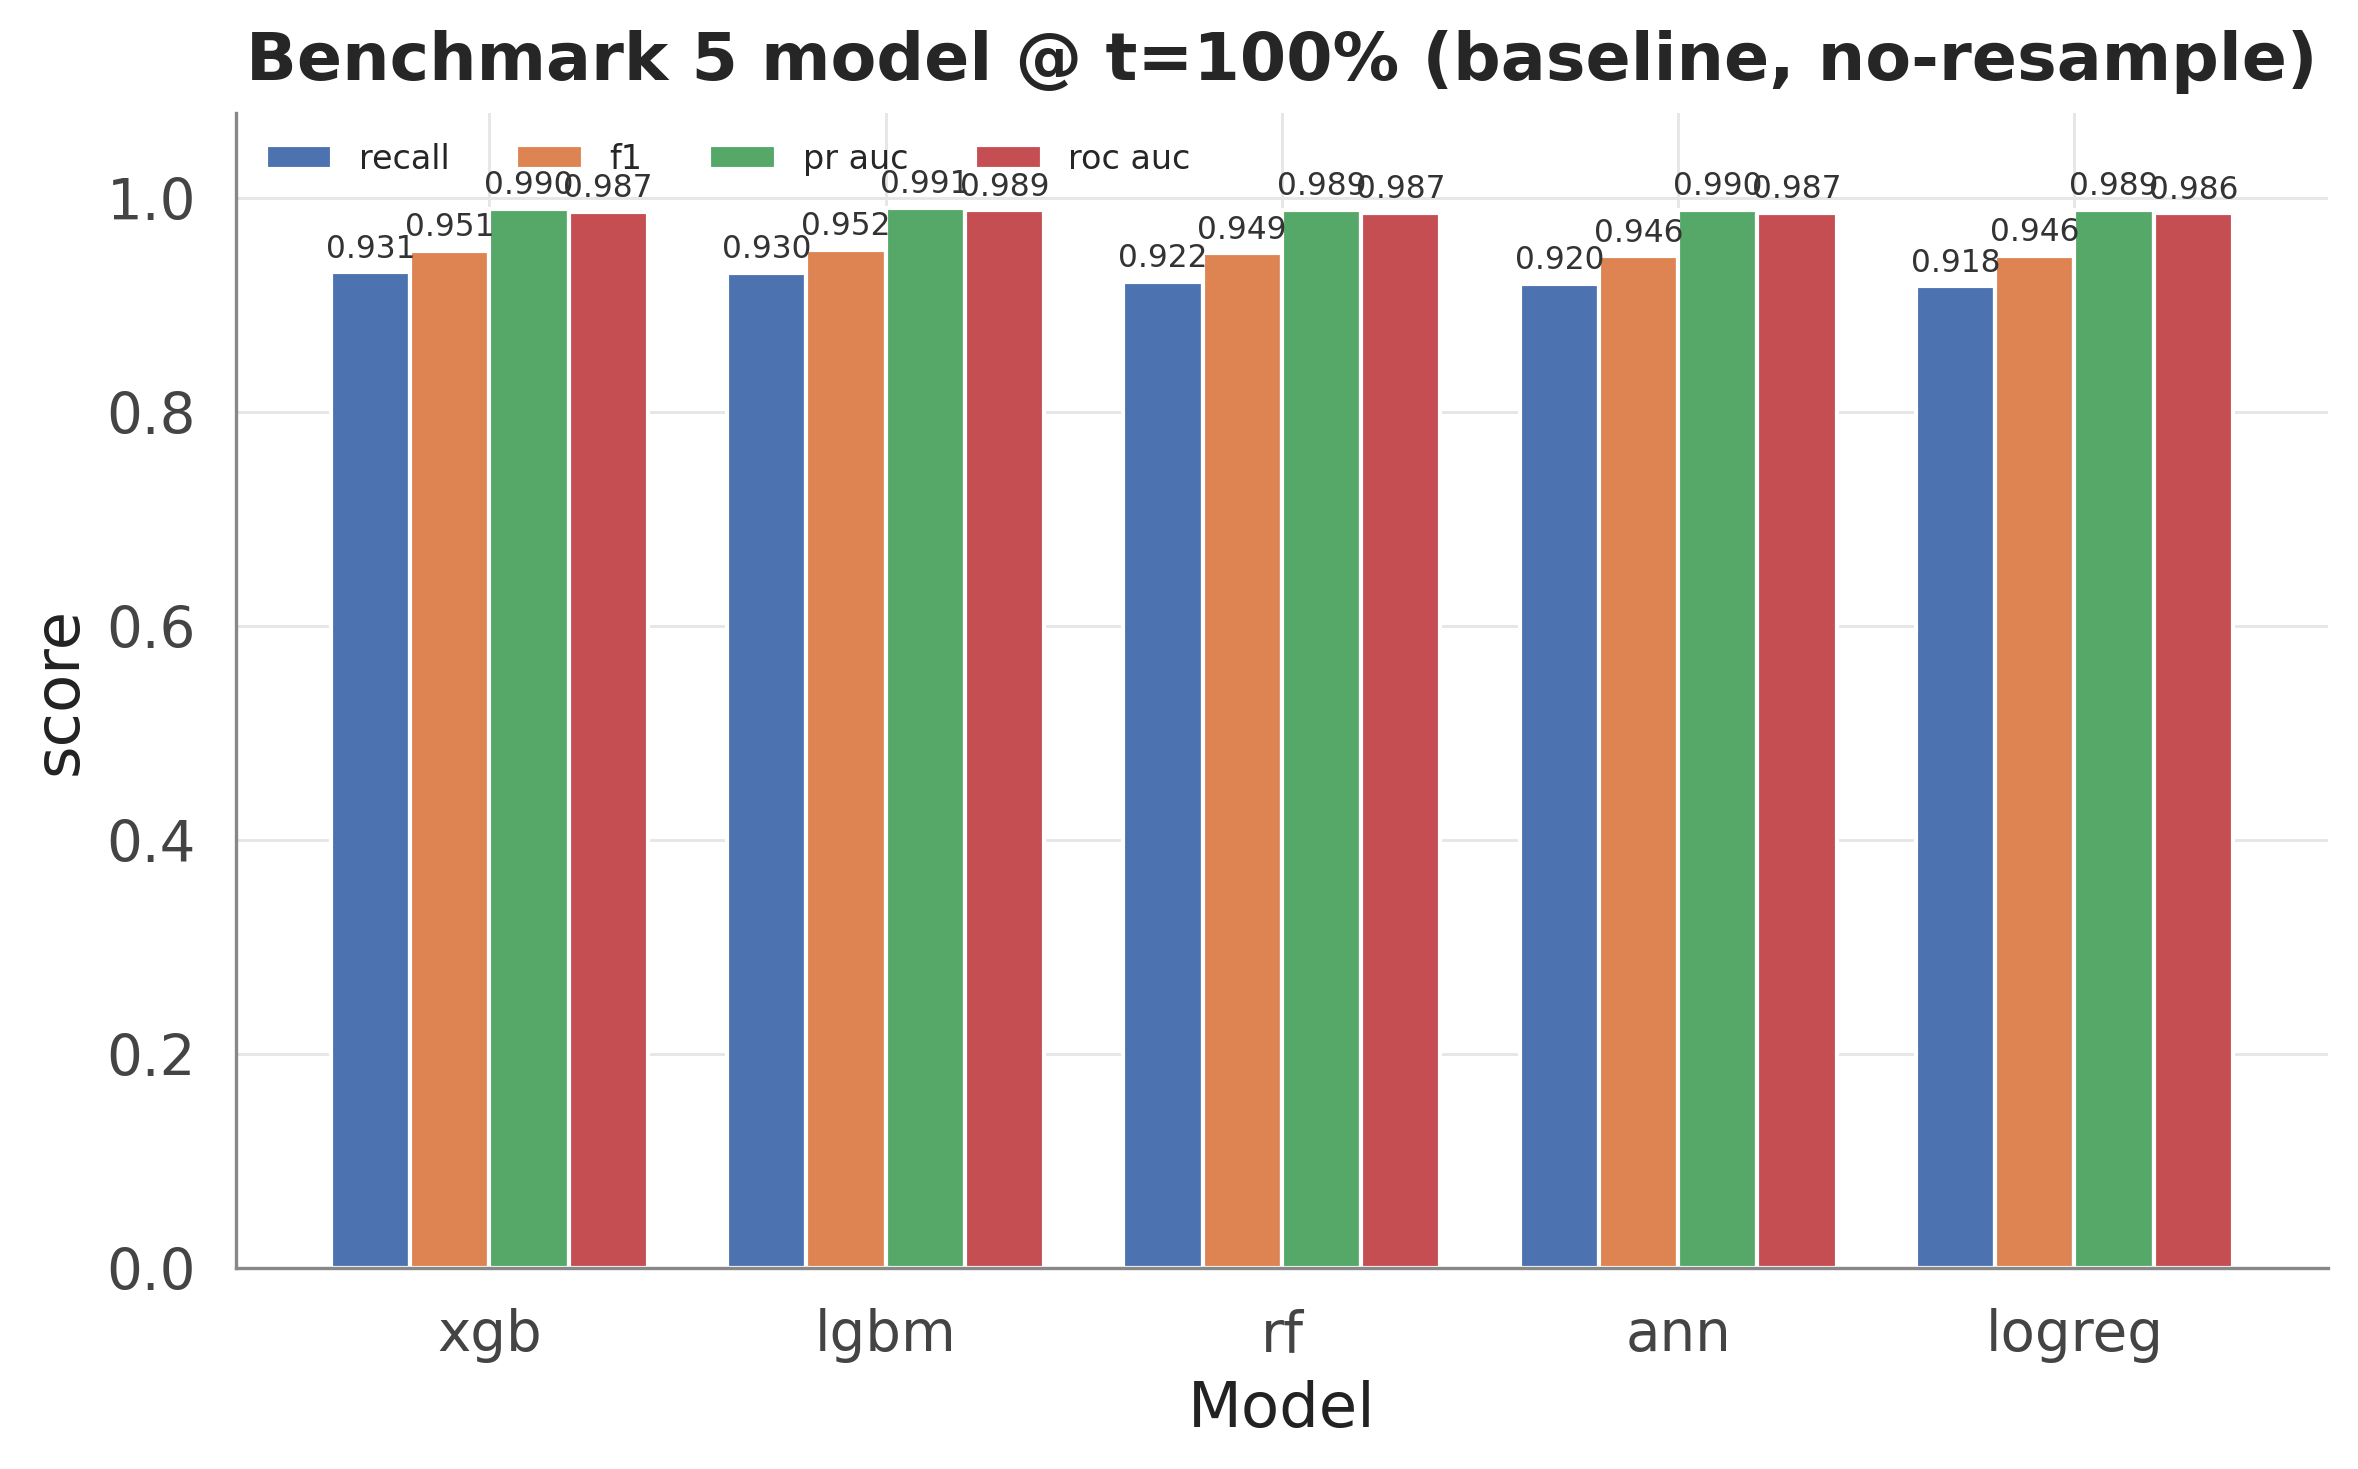
\includegraphics[height=0.82\textheight]{model_benchmark_baseline.png}
\end{frame}

\begin{frame}{4.3 · Bảng bảy chỉ số (baseline không tái lấy mẫu, sinh từ CSV)}
\centering\small
\textbf{XGBoost}: recall \textbf{0.931}; F1 \textbf{0.951}; PR-AUC \textbf{0.990}; Brier 0.038 (giá trị thấp là tốt)\\[2mm]
\begin{tabular}{@{}lcccccc@{}}
\toprule
\textbf{Mô hình} & \textbf{Recall} & \textbf{F1} & \textbf{PR-AUC} & \textbf{ROC-AUC} & \textbf{Precision} & \textbf{Brier}$\downarrow$ \\
\midrule
    XGBoost & 0.931 & 0.951 & 0.990 & 0.987 & 0.972 & 0.038 \\
    LightGBM & 0.930 & 0.952 & 0.991 & 0.989 & 0.974 & 0.037 \\
    Random Forest & 0.922 & 0.949 & 0.989 & 0.987 & 0.977 & 0.041 \\
    ANN (MLP) & 0.920 & 0.946 & 0.990 & 0.987 & 0.973 & 0.041 \\
    Logistic Regression & 0.918 & 0.946 & 0.989 & 0.986 & 0.976 & 0.041 \\
\bottomrule
\end{tabular}
\vspace{3mm}
\begin{itemize}\small
  \item Ba mô hình họ cây đạt kết quả rất gần nhau; Logistic Regression xếp cuối nhưng không kém xa, cho thấy tín hiệu trong đặc trưng mạnh và phần lớn tách được tuyến tính.
  \item Khoảng cách giữa các mô hình nhỏ; cần kiểm chứng xem thứ hạng có ý nghĩa thống kê hay chỉ là kết quả ngẫu nhiên của một lần phân chia dữ liệu.
\end{itemize}
\end{frame}

\begin{frame}{4.3 · Ma trận nhầm lẫn của mô hình được chọn (t=100\%, ngưỡng 0,50)}
\centering
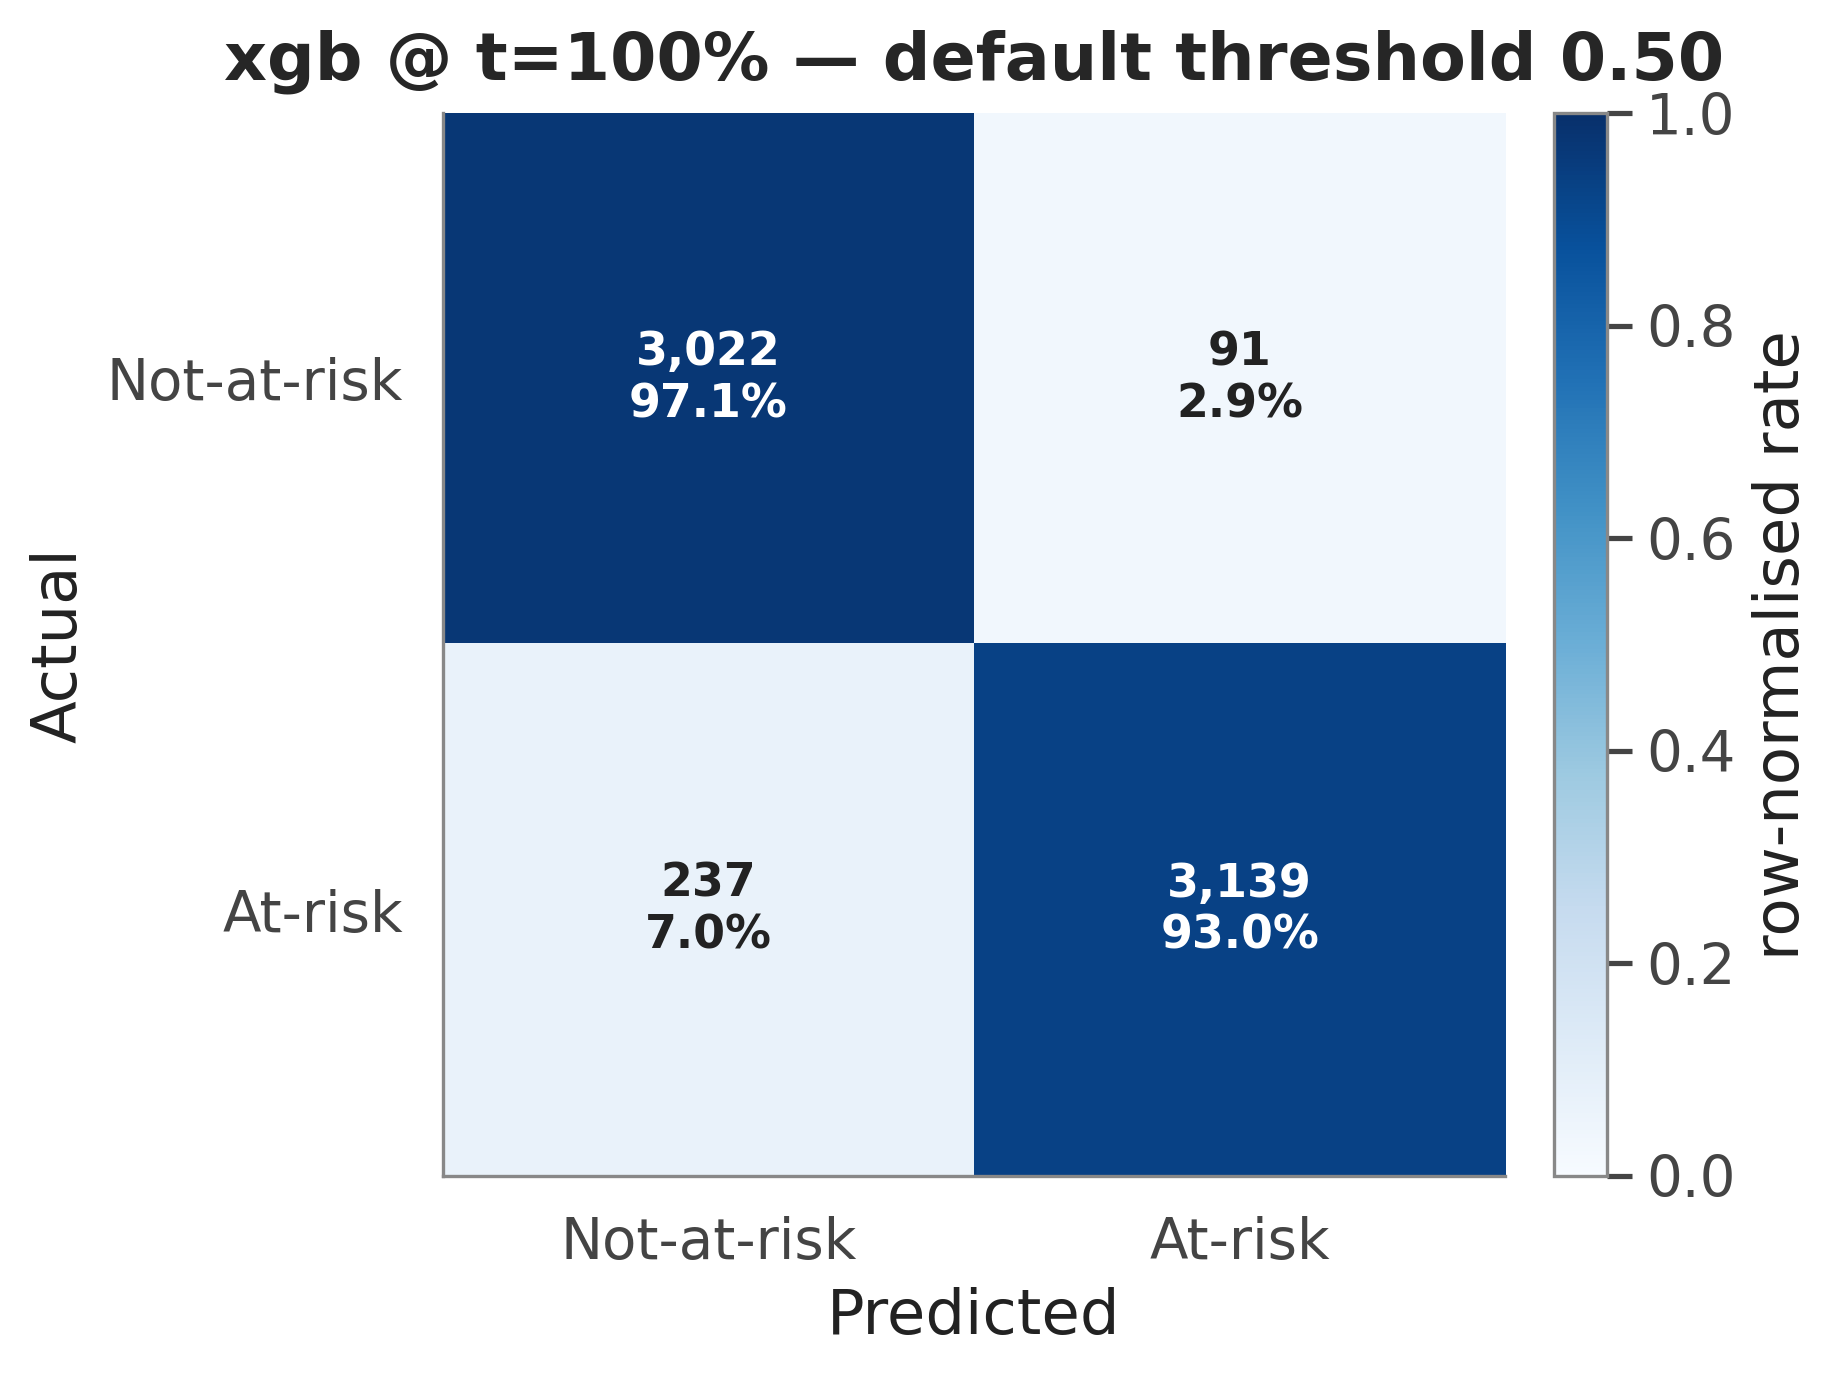
\includegraphics[height=0.74\textheight]{confusion_default_t100.png}\\
{\small Mô hình XGBoost của pipeline chuẩn (có SMOTE): recall 0,930, tỉ lệ bỏ sót lớp nguy cơ 7,0\%. Baseline không tái lấy mẫu ở bảng trước đạt recall 0,931; hai giá trị chênh nhau không đáng kể.}
\end{frame}

\begin{frame}{4.4 · Kiểm chứng thứ nhất: kiểm định chéo 5 fold $\times$ 5 seed}
\centering\small
\begin{tabular}{@{}lccc@{}}
\toprule
\textbf{Mô hình} & \textbf{Recall ($\mu\pm\sigma$)} & \textbf{F1 ($\mu\pm\sigma$)} & \textbf{PR-AUC ($\mu\pm\sigma$)} \\
\midrule
    XGBoost & 0.9309 $\pm$ 0.0047 & 0.9507 $\pm$ 0.0032 & 0.9901 $\pm$ 0.0008 \\
    LightGBM & 0.9295 $\pm$ 0.0060 & 0.9516 $\pm$ 0.0036 & 0.9907 $\pm$ 0.0008 \\
    ANN (MLP) & 0.9245 $\pm$ 0.0081 & 0.9463 $\pm$ 0.0038 & 0.9891 $\pm$ 0.0009 \\
    Random Forest & 0.9202 $\pm$ 0.0051 & 0.9489 $\pm$ 0.0030 & 0.9889 $\pm$ 0.0009 \\
    Logistic Regression & 0.9180 $\pm$ 0.0054 & 0.9452 $\pm$ 0.0033 & 0.9887 $\pm$ 0.0010 \\
\bottomrule
\end{tabular}
\vspace{3mm}
\begin{itemize}\small
  \item Hai mươi lăm lần huấn luyện cho mỗi mô hình; tiền xử lý và cân bằng lớp được lặp lại bên trong từng fold; các fold gộp theo sinh viên nên không phát sinh rò rỉ.
  \item Độ lệch chuẩn nhỏ so với chênh lệch giữa các mô hình; thứ hạng theo kiểm định chéo trùng với thứ hạng trên tập kiểm tra, do đó kết quả của một lần phân chia không phải điểm dị thường.
\end{itemize}
\end{frame}

\begin{frame}{4.4 · Độ bất định của ước lượng kiểm định chéo}
\centering
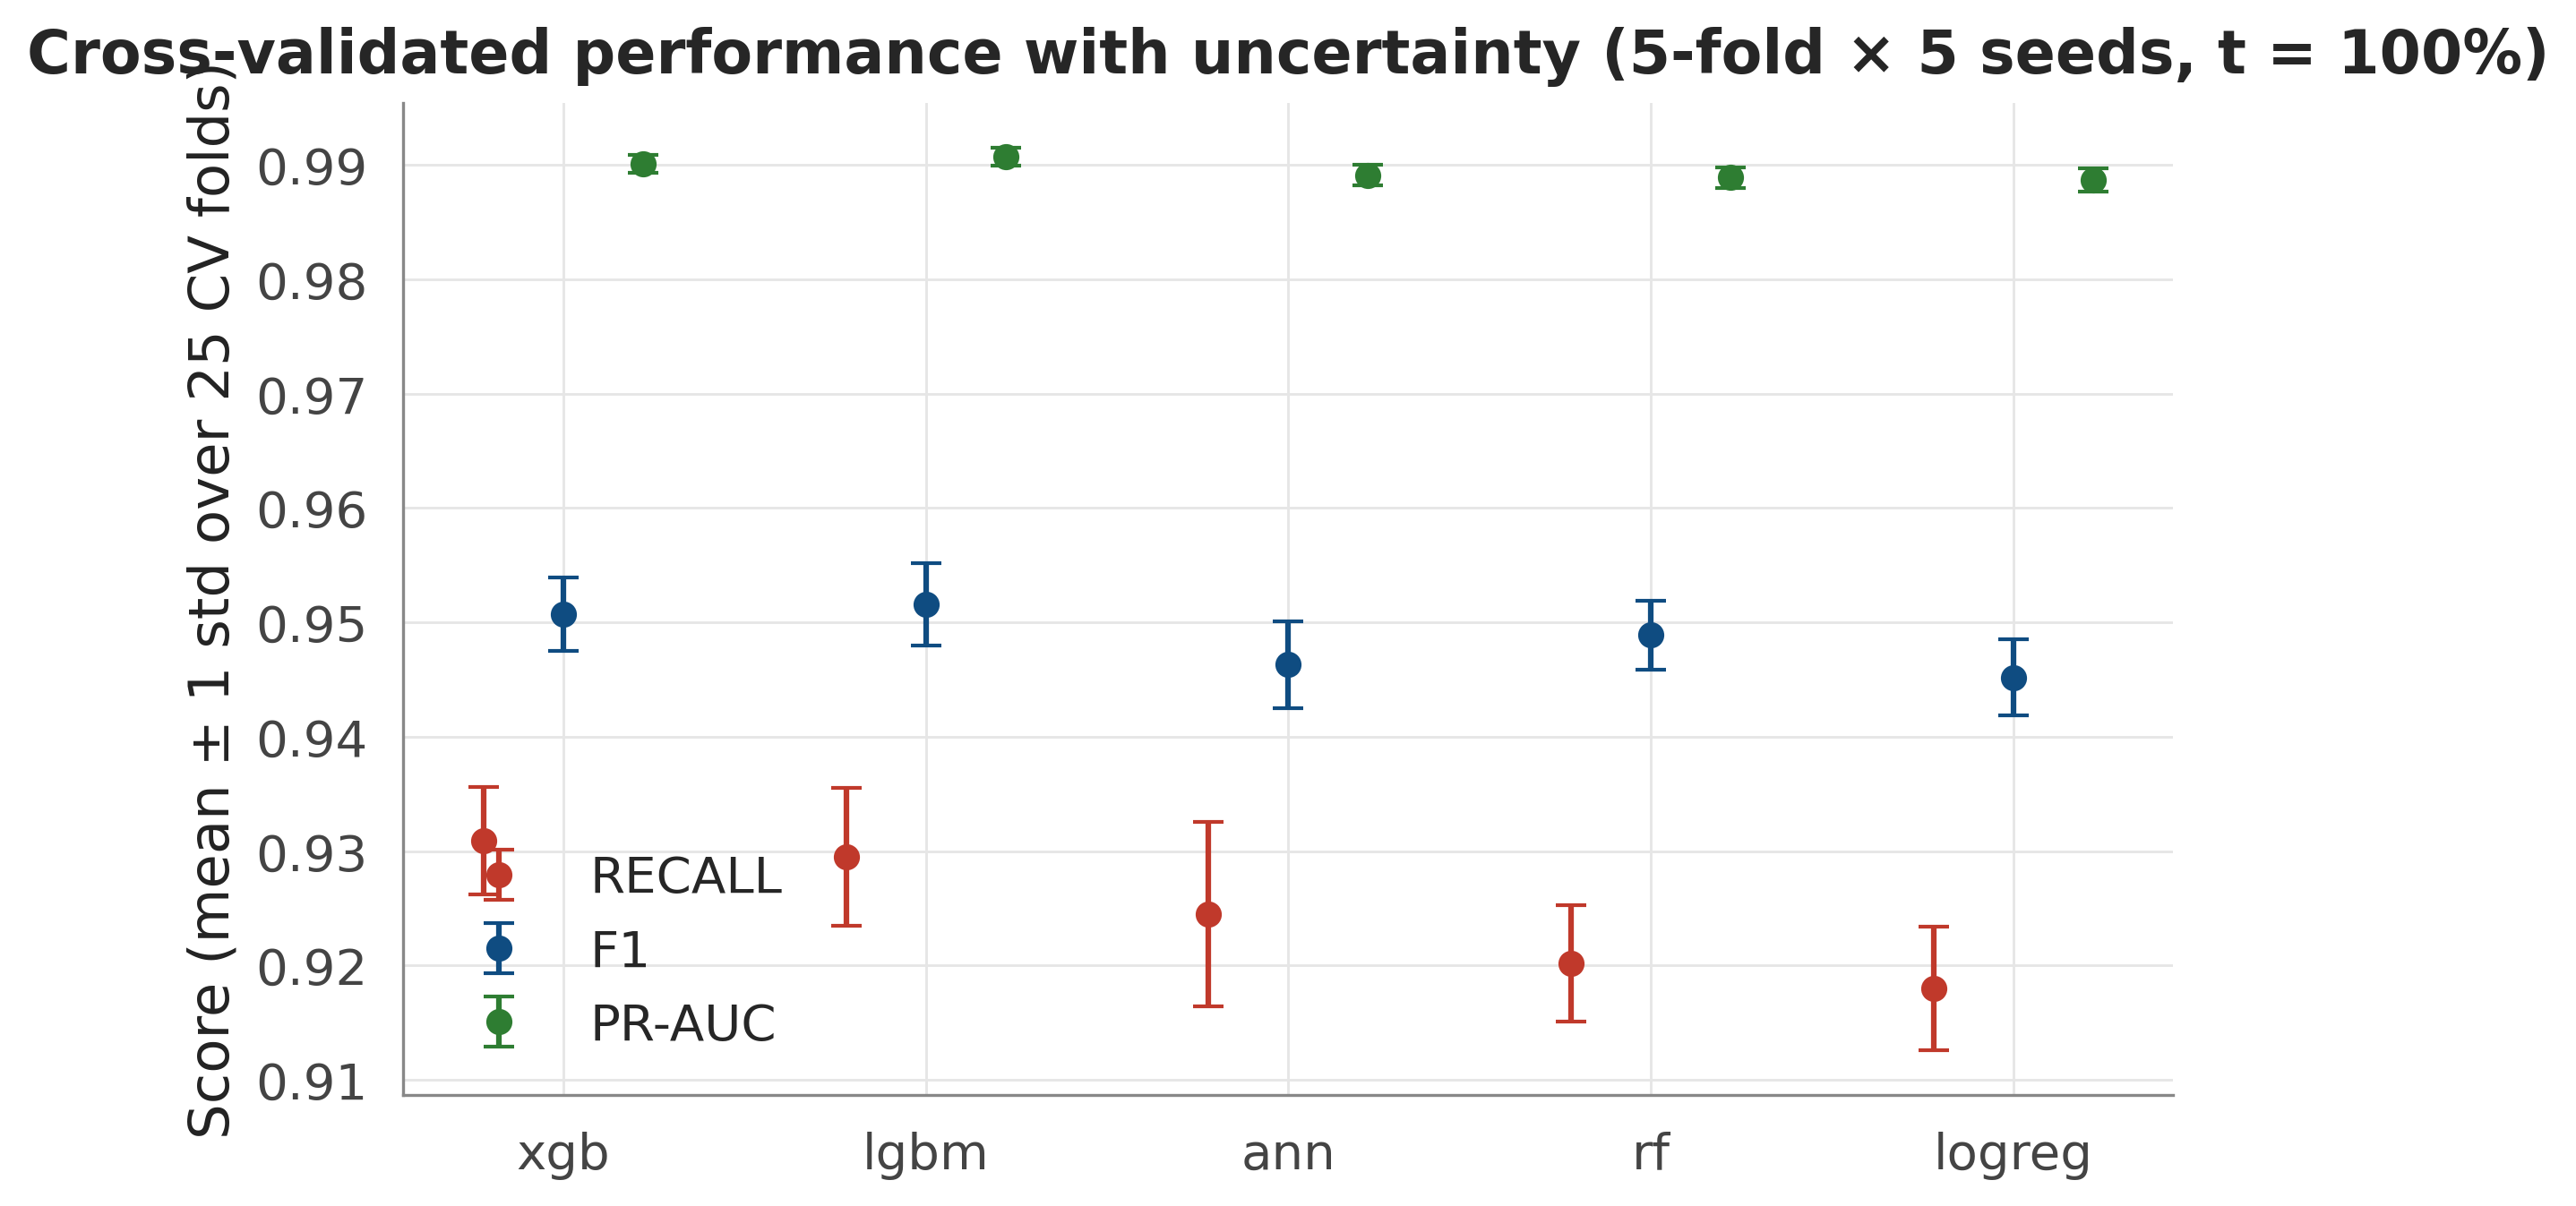
\includegraphics[height=0.78\textheight]{cv_uncertainty.png}\\
{\small Chênh lệch giữa các mô hình lớn hơn biến thiên nội tại của từng mô hình (trung bình $\pm$ 1 độ lệch chuẩn trên 25 fold).}
\end{frame}

\begin{frame}{4.4 · Kiểm chứng thứ hai: kiểm định thống kê trên 25 fold ghép cặp}
\centering\small
\begin{tabular}{@{}llcc@{}}
\toprule
\textbf{Chỉ số} & \textbf{Mô hình tốt nhất (mean rank)} & \textbf{Friedman $\chi^2$} & \textbf{p-value} \\
\midrule
    recall & XGBoost & 73.8 & $3.5\times 10^{-15}$ \\
    f1 & LightGBM & 83.8 & $2.7\times 10^{-17}$ \\
    pr\_auc & LightGBM & 82.6 & $4.9\times 10^{-17}$ \\
    roc\_auc & LightGBM & 77.7 & $5.4\times 10^{-16}$ \\
\bottomrule
\end{tabular}
\vspace{3mm}
\begin{itemize}\small
  \item Kiểm định Friedman bác bỏ giả thuyết các mô hình tương đương ở mọi chỉ số với mức ý nghĩa rất cao.
  \item Kiểm định hậu nghiệm Wilcoxon với hiệu chỉnh Holm cho recall: XGBoost cao hơn có ý nghĩa thống kê so với \textbf{4/4} mô hình còn lại; LightGBM dẫn đầu các chỉ số tổng hợp (F1, PR-AUC, ROC-AUC).
  \item XGBoost được chọn làm mô hình chính do khung đánh giá ưu tiên recall và do phần giải thích (RQ2) yêu cầu SHAP TreeExplainer chính xác.
\end{itemize}
\end{frame}

\begin{frame}{4.5 · Tinh chỉnh siêu tham số}
\centering\small
RandomizedSearchCV; 40 cấu hình cho mỗi mô hình; kiểm định chéo 5 fold gộp theo sinh viên; tối ưu PR-AUC; SMOTE trong từng fold\\[2mm]
\begin{tabular}{@{}lcccc@{}}
\toprule
 & \multicolumn{2}{c}{\textbf{PR-AUC}} & \multicolumn{2}{c}{\textbf{Recall}} \\
\textbf{Mô hình và mốc} & gốc & sau tinh chỉnh & gốc & sau tinh chỉnh \\
\midrule
    XGBoost tại t=40\% & 0.9428 & 0.9479 & 0.8107 & 0.8042 \\
    XGBoost tại t=100\% & 0.9902 & 0.9914 & 0.9298 & 0.9274 \\
    LightGBM tại t=40\% & 0.9473 & 0.9473 & 0.8095 & 0.8110 \\
    LightGBM tại t=100\% & 0.9913 & 0.9910 & 0.9295 & 0.9301 \\
\bottomrule
\end{tabular}
\vspace{3mm}
\begin{itemize}\small
  \item Random search được chọn thay cho grid search (chi phí tổ hợp lớn) và Bayesian optimisation (lợi ích không tương xứng ở quy mô 40 cấu hình).
  \item Với XGBoost tại t=100\%: PR-AUC tăng 0.0012 nhưng recall giảm từ 0.9298 xuống 0.9274. Mức cải thiện không tương xứng với chi phí tái lập của một cấu hình riêng, do đó \textbf{cấu hình gần mặc định được giữ nguyên}.
\end{itemize}
\end{frame}

\begin{frame}{RQ3 · Ảnh hưởng của bốn chiến lược cân bằng lớp}
\centering
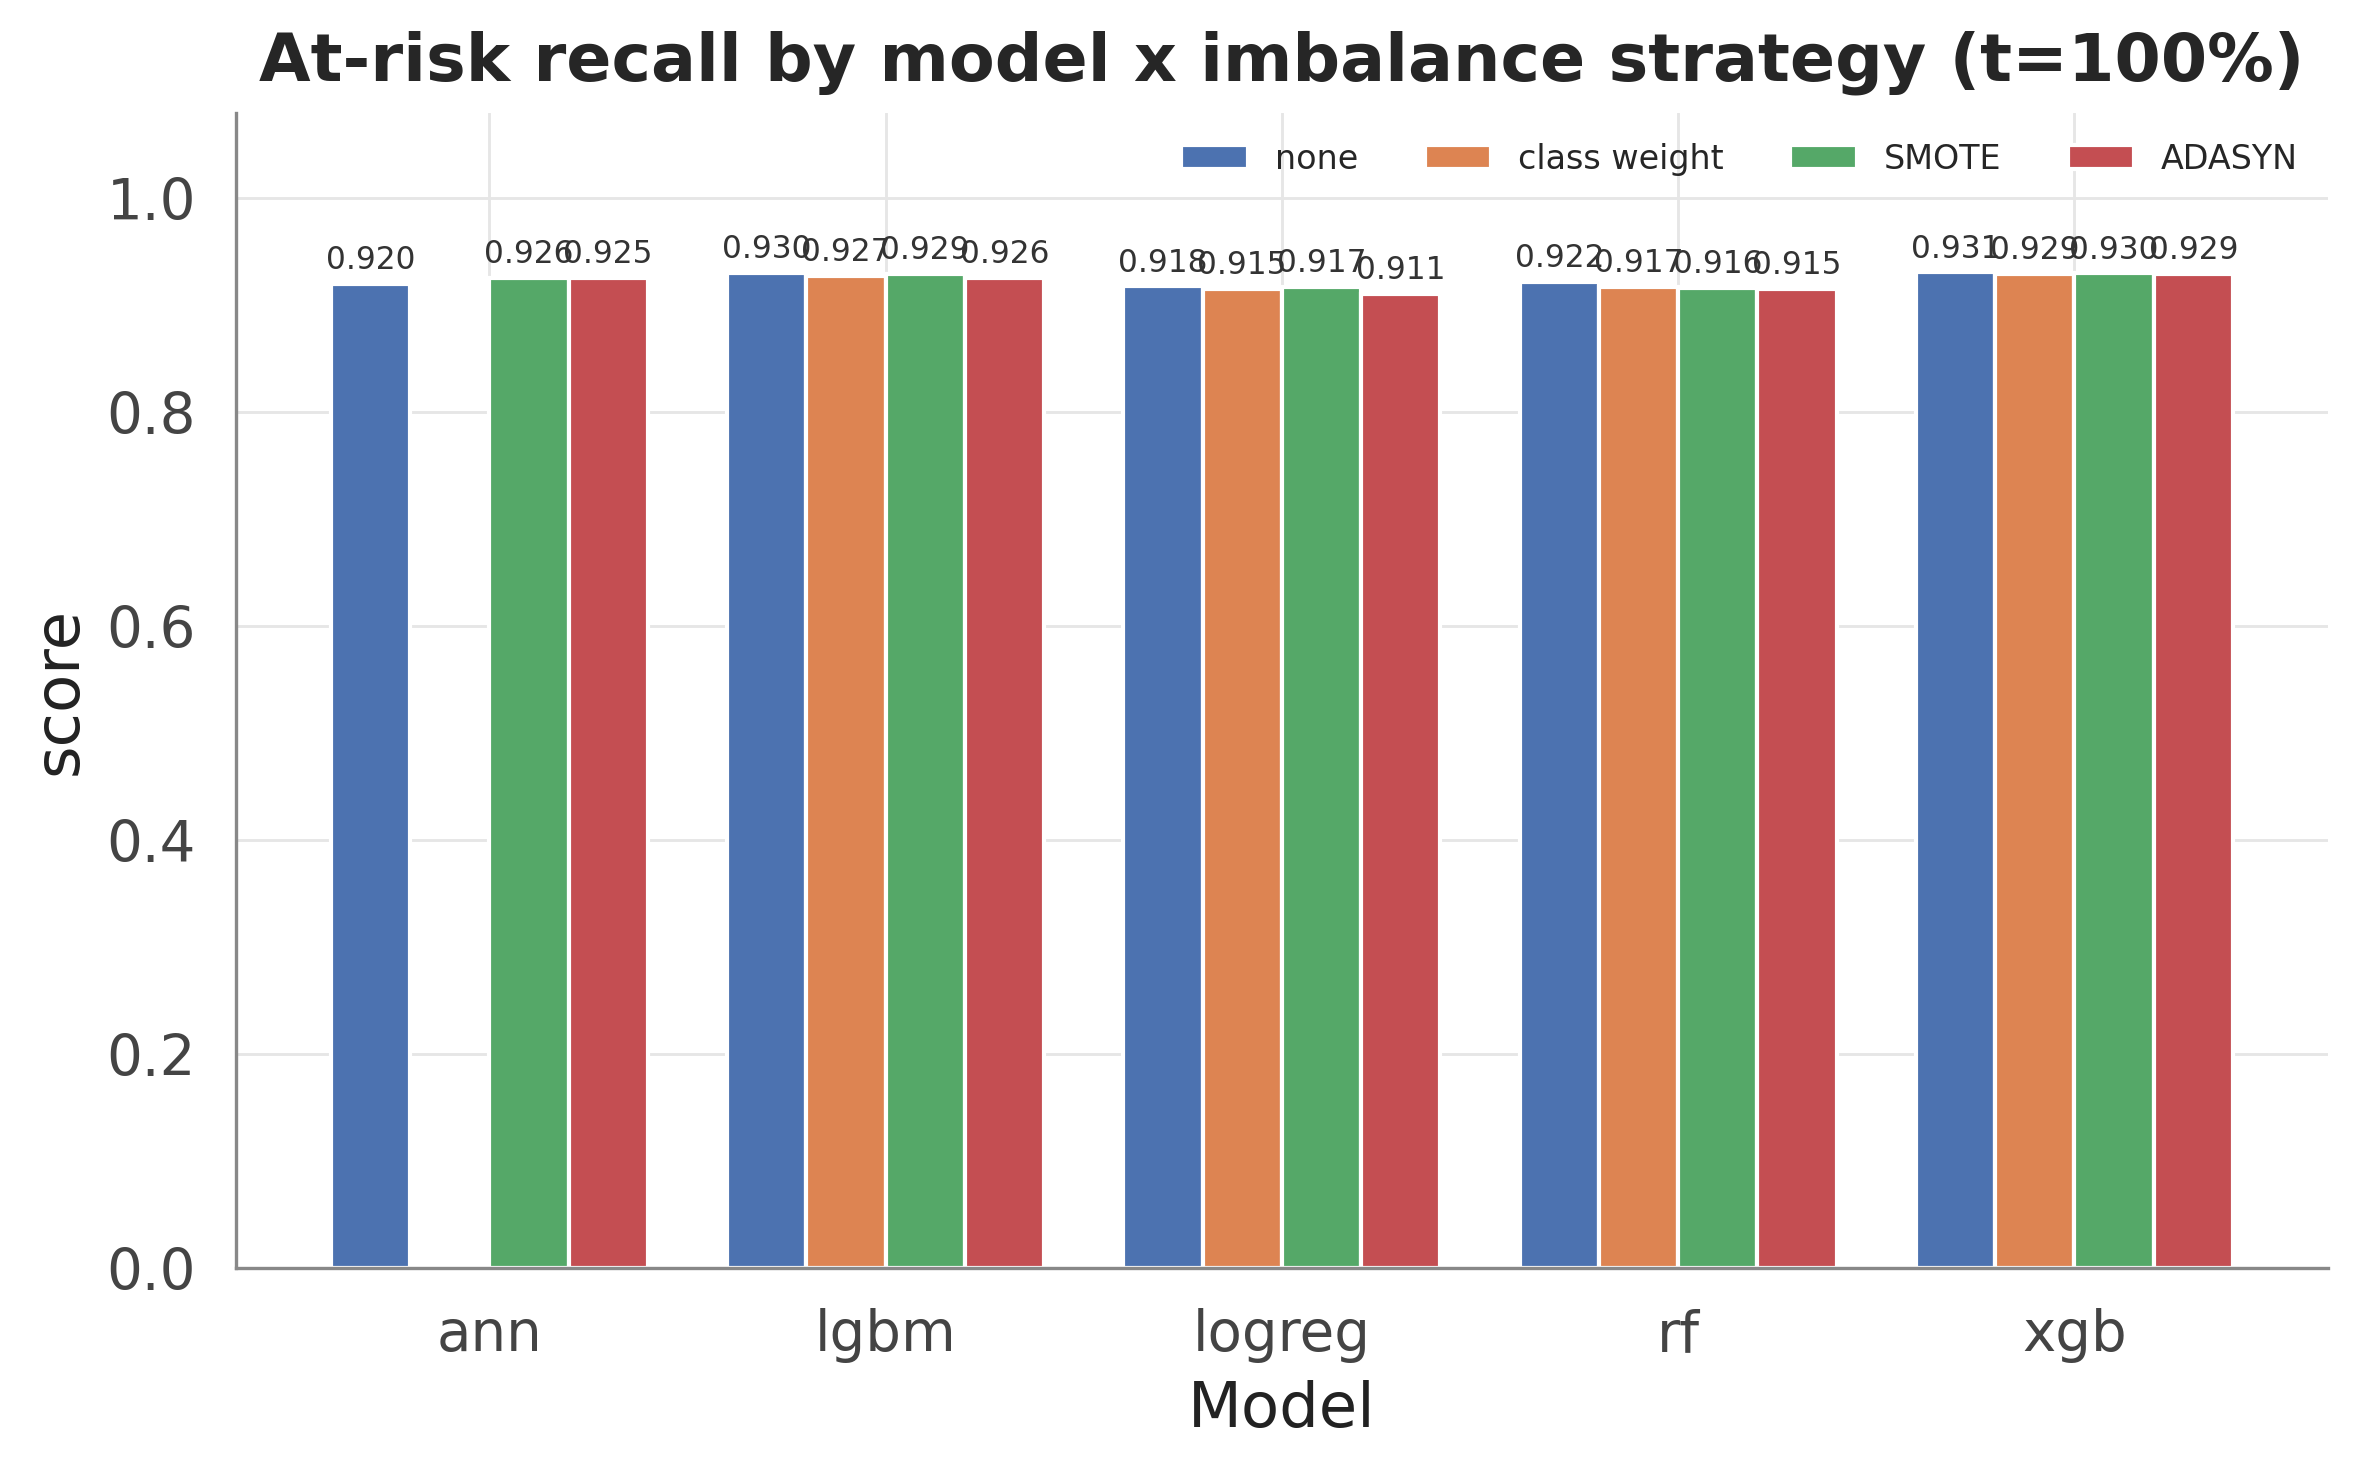
\includegraphics[height=0.82\textheight]{imbalance_recall_by_model.png}
\end{frame}

\begin{frame}{RQ3 · Recall theo mô hình và chiến lược cân bằng (t=100\%)}
\centering\small
\begin{tabular}{@{}lccccc@{}}
\toprule
\textbf{Mô hình} & \textbf{none} & \textbf{class\_weight} & \textbf{SMOTE} & \textbf{ADASYN} & \textbf{Chênh lệch lớn nhất} \\
\midrule
    XGBoost & 0.9307 & 0.9295 & 0.9298 & 0.9292 & 0.0015 \\
    LightGBM & 0.9301 & 0.9274 & 0.9295 & 0.9259 & 0.0042 \\
    Random Forest & 0.9221 & 0.9171 & 0.9165 & 0.9153 & 0.0068 \\
    ANN (MLP) & 0.9200 & không hỗ trợ & 0.9259 & 0.9254 & 0.0059 \\
    Logistic Regression & 0.9177 & 0.9153 & 0.9171 & 0.9108 & 0.0069 \\
\bottomrule
\end{tabular}
\vspace{3mm}
\begin{itemize}\small
  \item Lớp nguy cơ chiếm 52,8\% (tỉ lệ mất cân bằng 1,12), tức đa số nhẹ; RQ3 vì vậy được đặt như một câu hỏi về tính bền vững của kết quả, không phải về khắc phục lớp thiểu số hiếm. ANN không hỗ trợ class\_weight, nên lưới thử nghiệm gồm 19 cấu hình.
  \item Chênh lệch recall lớn nhất giữa bốn chiến lược trên mọi mô hình là \textbf{0.0069}: kết quả không phụ thuộc cách xử lý mất cân bằng; pipeline giữ SMOTE theo đề cương đã duyệt.
\end{itemize}
\end{frame}

\begin{frame}{RQ1 · Hiệu năng theo sáu mốc thời gian (quần thể đầy đủ)}
\centering
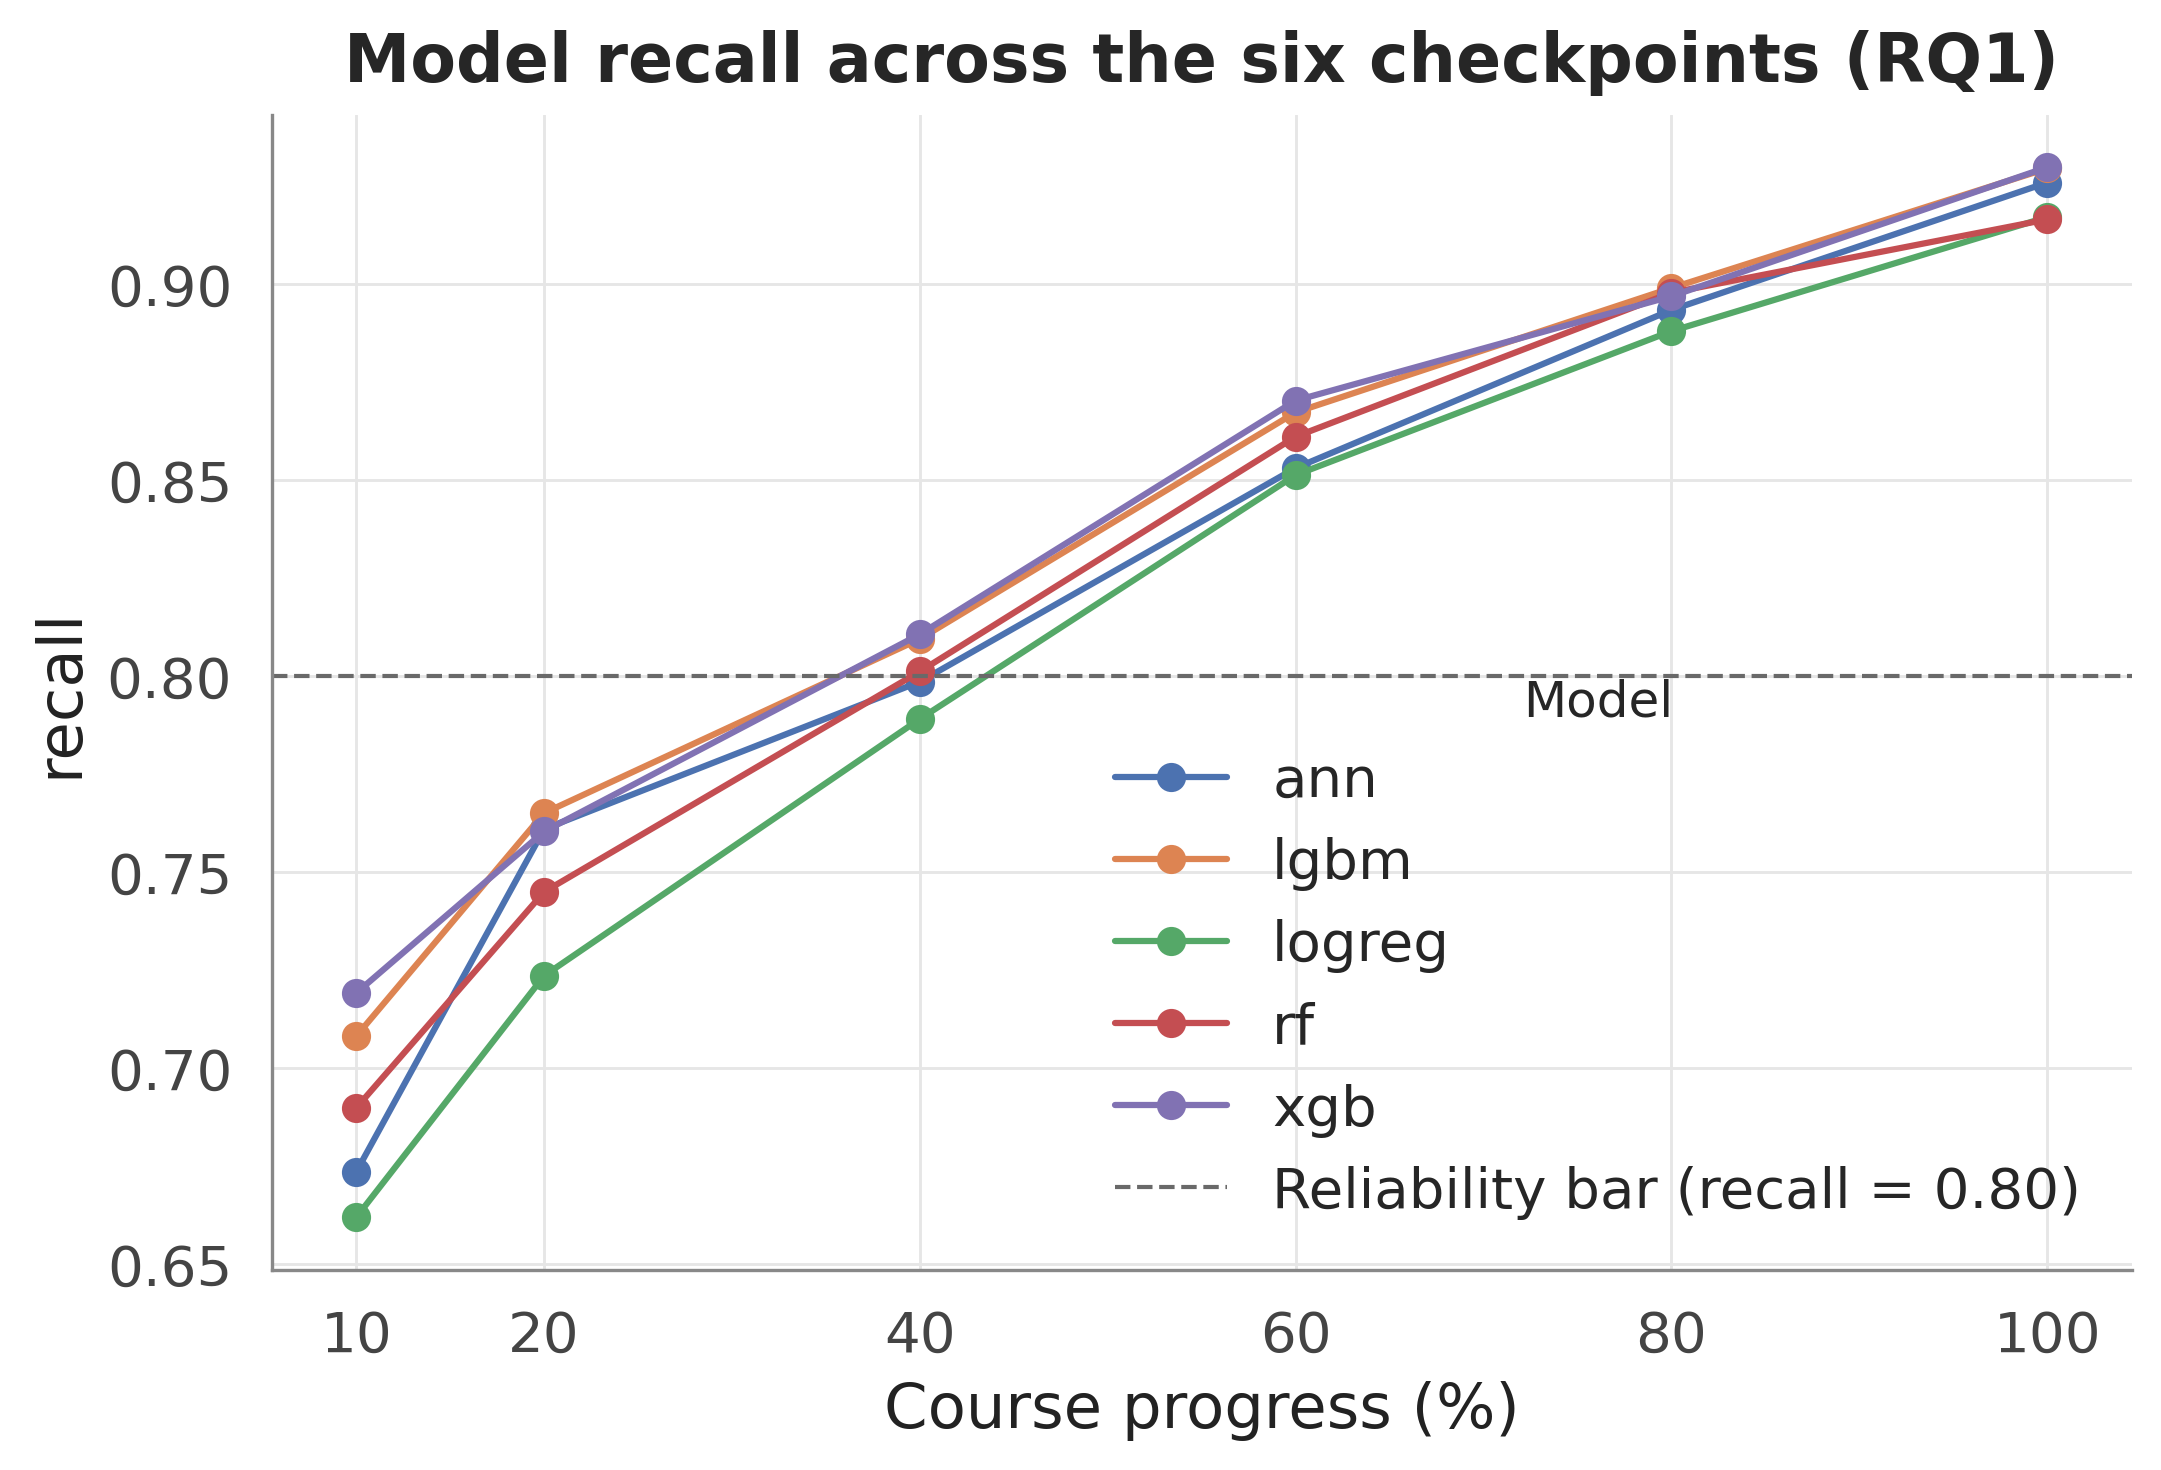
\includegraphics[width=0.49\textwidth]{time_aware_recall.png}\hfill
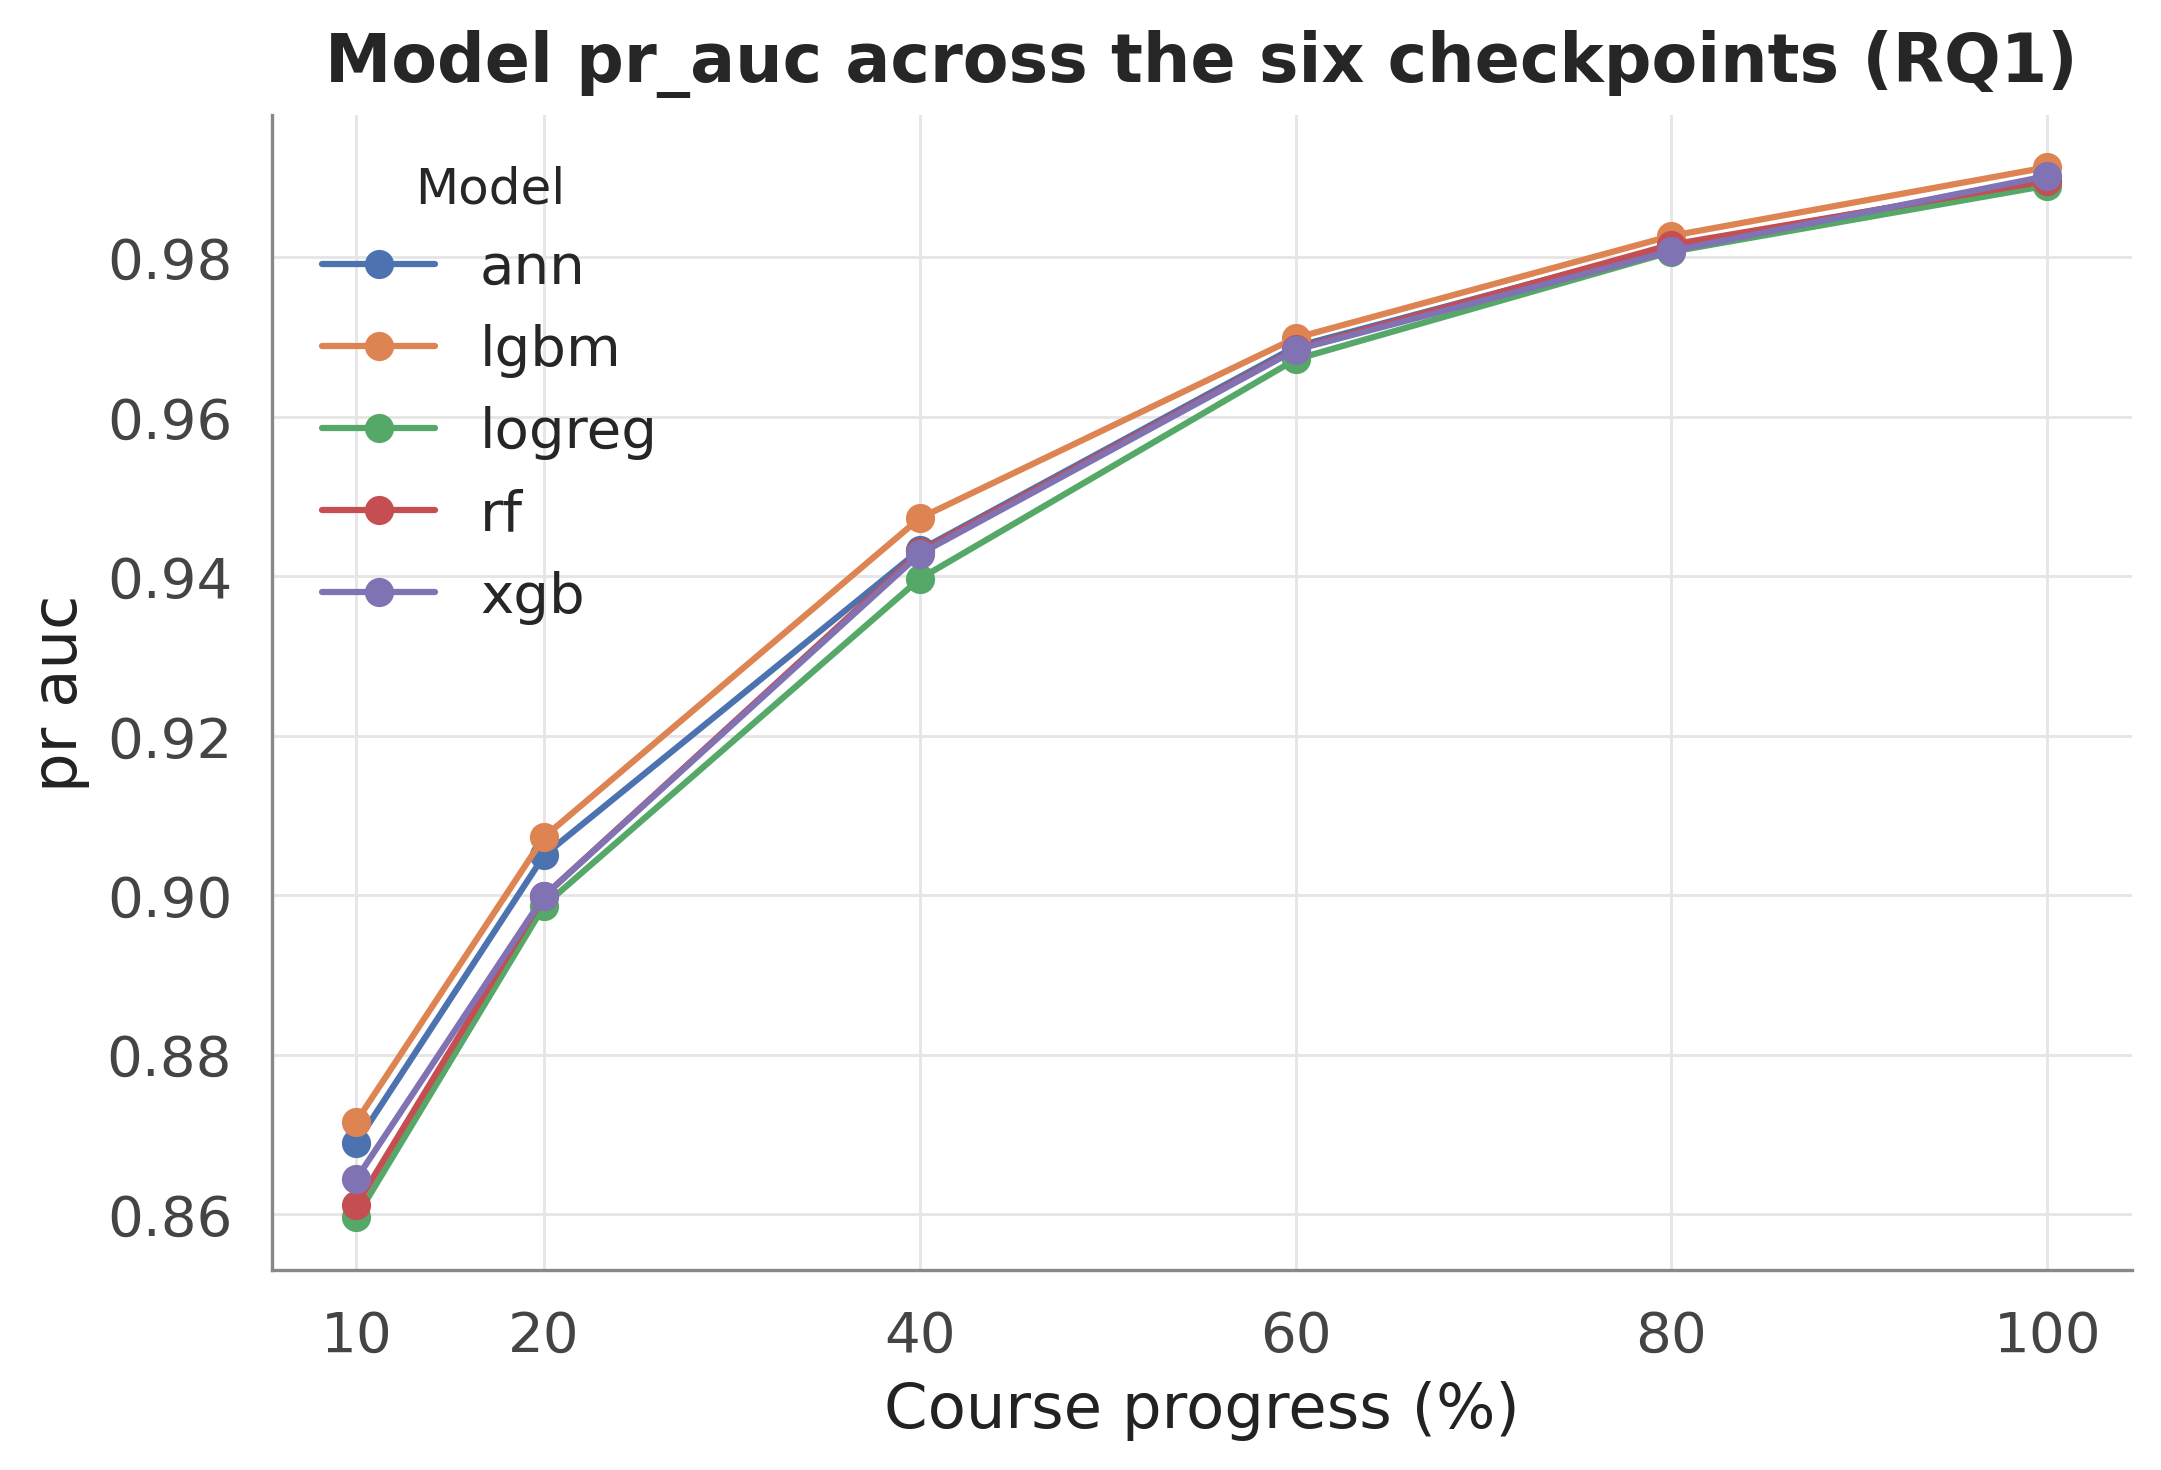
\includegraphics[width=0.49\textwidth]{time_aware_pr_auc.png}\\
{\small Recall (trái) chỉ vượt tiêu chí 0,80 từ t=40\%; PR-AUC (phải) vượt tiêu chí 0,80 tại mọi mốc, do đó không vẽ đường tham chiếu. Hai biểu đồ là hai vế của cùng một tiêu chí tin cậy.}
\end{frame}

\begin{frame}{RQ1 · Mô hình tốt nhất theo từng mốc (quần thể đầy đủ)}
\centering\small
\begin{tabular}{@{}llcccc@{}}
\toprule
\textbf{Mốc} & \textbf{Mô hình tốt nhất} & \textbf{Recall} & \textbf{PR-AUC} & \textbf{F1} & \textbf{Tiêu chí} \\
\midrule
    10\% & XGBoost & 0.719 & 0.864 & 0.747 & Chưa đạt \\
    20\% & LightGBM & 0.765 & 0.907 & 0.800 & Chưa đạt \\
    40\% & XGBoost & 0.811 & 0.943 & 0.848 & Đạt \\
    60\% & XGBoost & 0.870 & 0.968 & 0.896 & Đạt \\
    80\% & LightGBM & 0.899 & 0.983 & 0.928 & Đạt \\
    100\% & XGBoost & 0.930 & 0.990 & 0.950 & Đạt \\
\bottomrule
\end{tabular}
\vspace{3mm}
\begin{itemize}\small
  \item XGBoost dẫn đầu recall tại các mốc 10, 40, 60, 100\%; LightGBM tại các mốc 20, 80\%. Hai mô hình boosting luân phiên dẫn đầu với chênh lệch nhỏ, củng cố kết luận rằng họ boosting, chứ không phải một thuật toán riêng lẻ, chiếm ưu thế.
  \item Tại t=40\%: recall 0.811 với khoảng tin cậy bootstrap 95\% [0.798, 0.824]. Khoảng này \textbf{chứa ngưỡng 0,80}, nên kết luận đạt chuẩn tại t=40\% chỉ ở mức ranh giới; từ t=60\% toàn bộ khoảng tin cậy nằm trên ngưỡng ([0.859, 0.882]).
\end{itemize}
\end{frame}

\begin{frame}{RQ1 · Quần thể đầy đủ bao gồm cả sinh viên đã rút trước mốc}
\centering
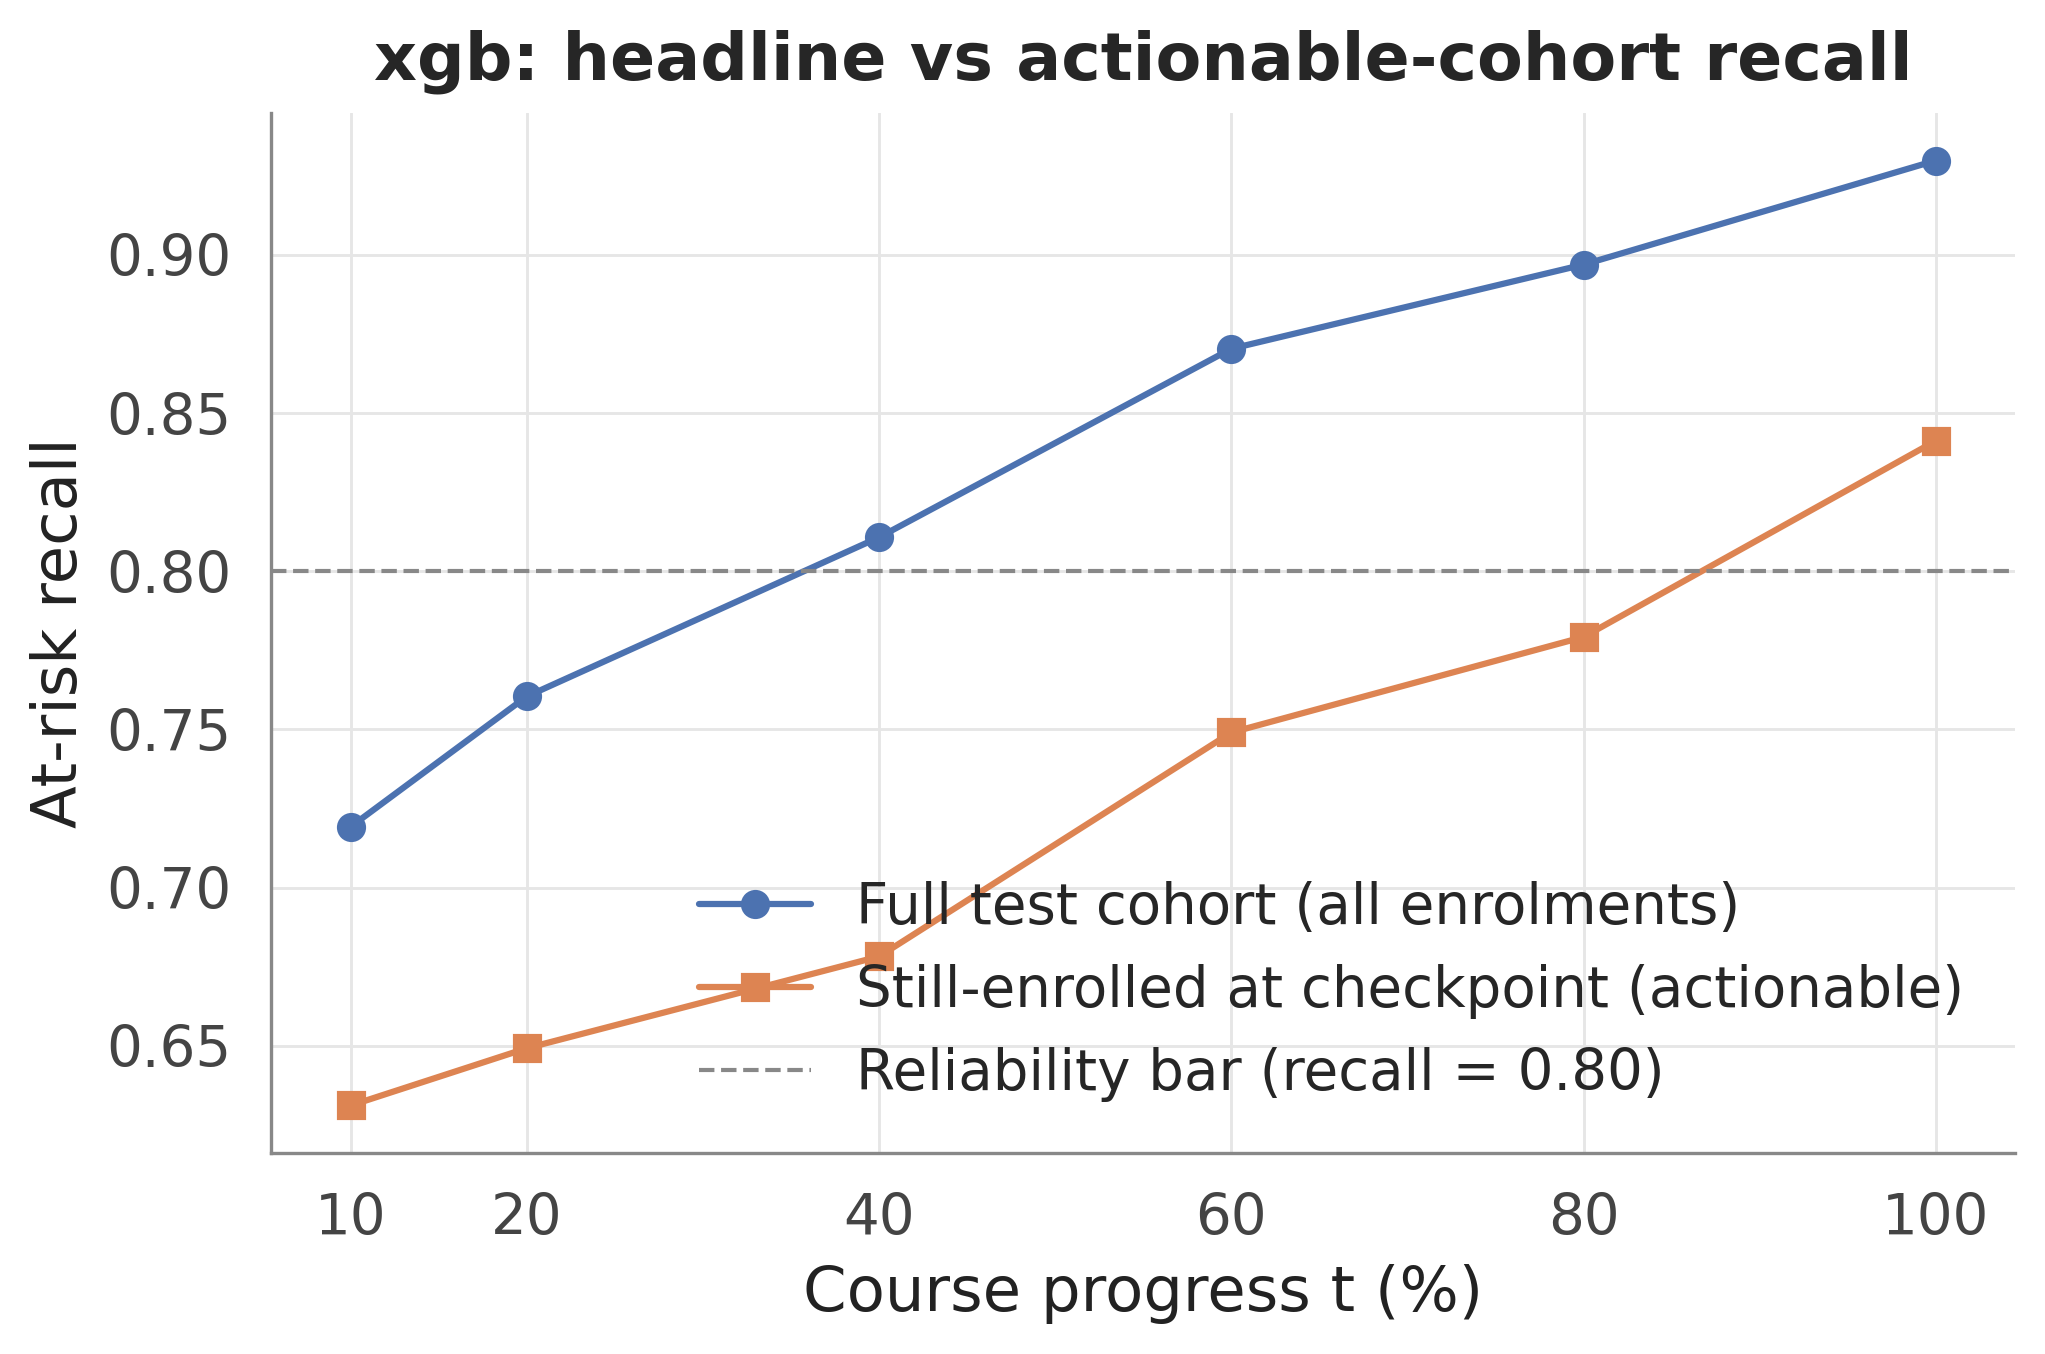
\includegraphics[height=0.78\textheight]{sensitivity_active_recall_xgb.png}
\end{frame}

\begin{frame}{RQ1 · Kết luận kép theo hai quần thể}
\centering\small
\begin{tabular}{@{}lccccc@{}}
\toprule
\textbf{Mốc} & \textbf{Recall đầy đủ} & \textbf{Recall còn theo học} & \textbf{Chênh lệch [KTC 95\%]} & \textbf{N còn theo học} & \textbf{Đã rút trước mốc} \\
\midrule
    10\% & 0.719 & 0.631 & 0.088 [0.080, 0.096] & 5,566 & 923 \\
    20\% & 0.760 & 0.649 & 0.111 [0.102, 0.120] & 5,359 & 1,130 \\
    40\% & 0.811 & 0.678 & 0.133 [0.122, 0.144] & 5,052 & 1,437 \\
    60\% & 0.870 & 0.749 & 0.121 [0.110, 0.133] & 4,802 & 1,687 \\
    80\% & 0.897 & 0.779 & 0.118 [0.106, 0.130] & 4,630 & 1,859 \\
    100\% & 0.930 & 0.841 & 0.089 [0.076, 0.101] & 4,536 & 1,953 \\
\bottomrule
\end{tabular}
\vspace{2mm}
\begin{itemize}\small
  \item Khoảng tin cậy của chênh lệch \textbf{không chứa 0 tại cả sáu mốc} (cận dưới nhỏ nhất 0.076): một phần recall của quần thể đầy đủ đến từ các sinh viên đã rút, tức là ghi nhận một kết cục đã xảy ra thay vì dự báo.
  \item Trên \textbf{quần thể đầy đủ} (khung so sánh với văn liệu): đạt chuẩn từ t=40\%, ở mức ranh giới. Trên \textbf{quần thể còn theo học} (khung can thiệp thực tế): tiêu chí chỉ đạt tại t=100\%, recall 0.841, khoảng tin cậy [0.821, 0.861].
  \item Đây không phải rò rỉ dữ liệu: nhãn không tham gia vào đặc trưng, và mức độ bất hoạt của sinh viên đã rút là hành vi quan sát thực. Đây là khác biệt về \textbf{định nghĩa quần thể} mà hai nghiên cứu nền không tách bạch.
\end{itemize}
\end{frame}

\begin{frame}{4.7 · Ngưỡng quyết định chọn trên tập validation}
\centering\small
\begin{tabular}{@{}lcccc@{}}
\toprule
\textbf{Chính sách} & \textbf{Ngưỡng} & \textbf{Recall (val)} & \textbf{Recall (test)} & \textbf{Precision (test)} \\
\midrule
    Ngưỡng mặc định (0,50) & 0.50 & 0.930 & 0.930 & 0.972 \\
    Tối ưu F1 & 0.56 & 0.926 & 0.926 & 0.975 \\
    Chỉ số Youden J & 0.56 & 0.926 & 0.926 & 0.975 \\
    Recall $\geq$ 0,9 & 0.86 & 0.901 & 0.900 & 0.993 \\
\bottomrule
\end{tabular}
\vspace{3mm}
\begin{itemize}\small
  \item Ngưỡng được chọn trên \textbf{dự đoán out-of-fold} của tập huấn luyện, cố định trước, sau đó đánh giá trên tập kiểm tra đúng một lần; quy trình này loại trừ việc tối ưu ngưỡng trên tập kiểm tra.
  \item Chính sách tối ưu F1 cho ngưỡng 0.56, gần ngưỡng mặc định 0,50; các kết quả ở những mục trước vì vậy không phải sản phẩm của việc lựa chọn ngưỡng.
  \item Chính sách recall $\geq$ 0,9: ngưỡng 0.86 đạt recall 0.900 với precision 0.993 trên tập kiểm tra. Các ngưỡng này \emph{chỉ được kiểm chứng cho XGBoost tại t=100\%}.
\end{itemize}
\end{frame}

\begin{frame}{4.8 · Hiệu năng phân tách theo nhóm nhân khẩu học (t=100\%, ngưỡng 0,50)}
\centering\small
\begin{tabular}{@{}lccc@{}}
\toprule
\textbf{Thuộc tính} & \textbf{Số nhóm} & \textbf{Chênh lệch recall} & \textbf{Chênh lệch FPR} \\
\midrule
    Mức nghèo khu vực (IMD) & 11 & 6.6 pp & 4.6 pp \\
    Vùng cư trú & 13 & 4.1 pp & 3.9 pp \\
    Học vấn đầu vào & 5 & 3.0 pp & 5.3 pp \\
    Giới tính & 2 & 2.6 pp & 0.2 pp \\
    Khuyết tật & 2 & 1.7 pp & 2.1 pp \\
    Nhóm tuổi & 2 & 1.6 pp & 0.7 pp \\
\bottomrule
\end{tabular}
\vspace{3mm}
\begin{itemize}\small
  \item Chỉ xét các nhóm có tối thiểu 50 sinh viên trong tập kiểm tra. Chênh lệch recall lớn nhất là \textbf{6.6 điểm phần trăm} (Mức nghèo khu vực (IMD)); recall của nhóm khai báo khuyết tật không thấp hơn nhóm còn lại.
  \item Đây là số liệu quan sát tại một mốc và một ngưỡng, không phải chứng nhận công bằng; hệ thống khi triển khai cần giám sát liên tục các chỉ số phân tách này.
\end{itemize}
\end{frame}

\begin{frame}{RQ2 · Đặc trưng nào ảnh hưởng lớn nhất đến dự đoán nguy cơ?}
\centering
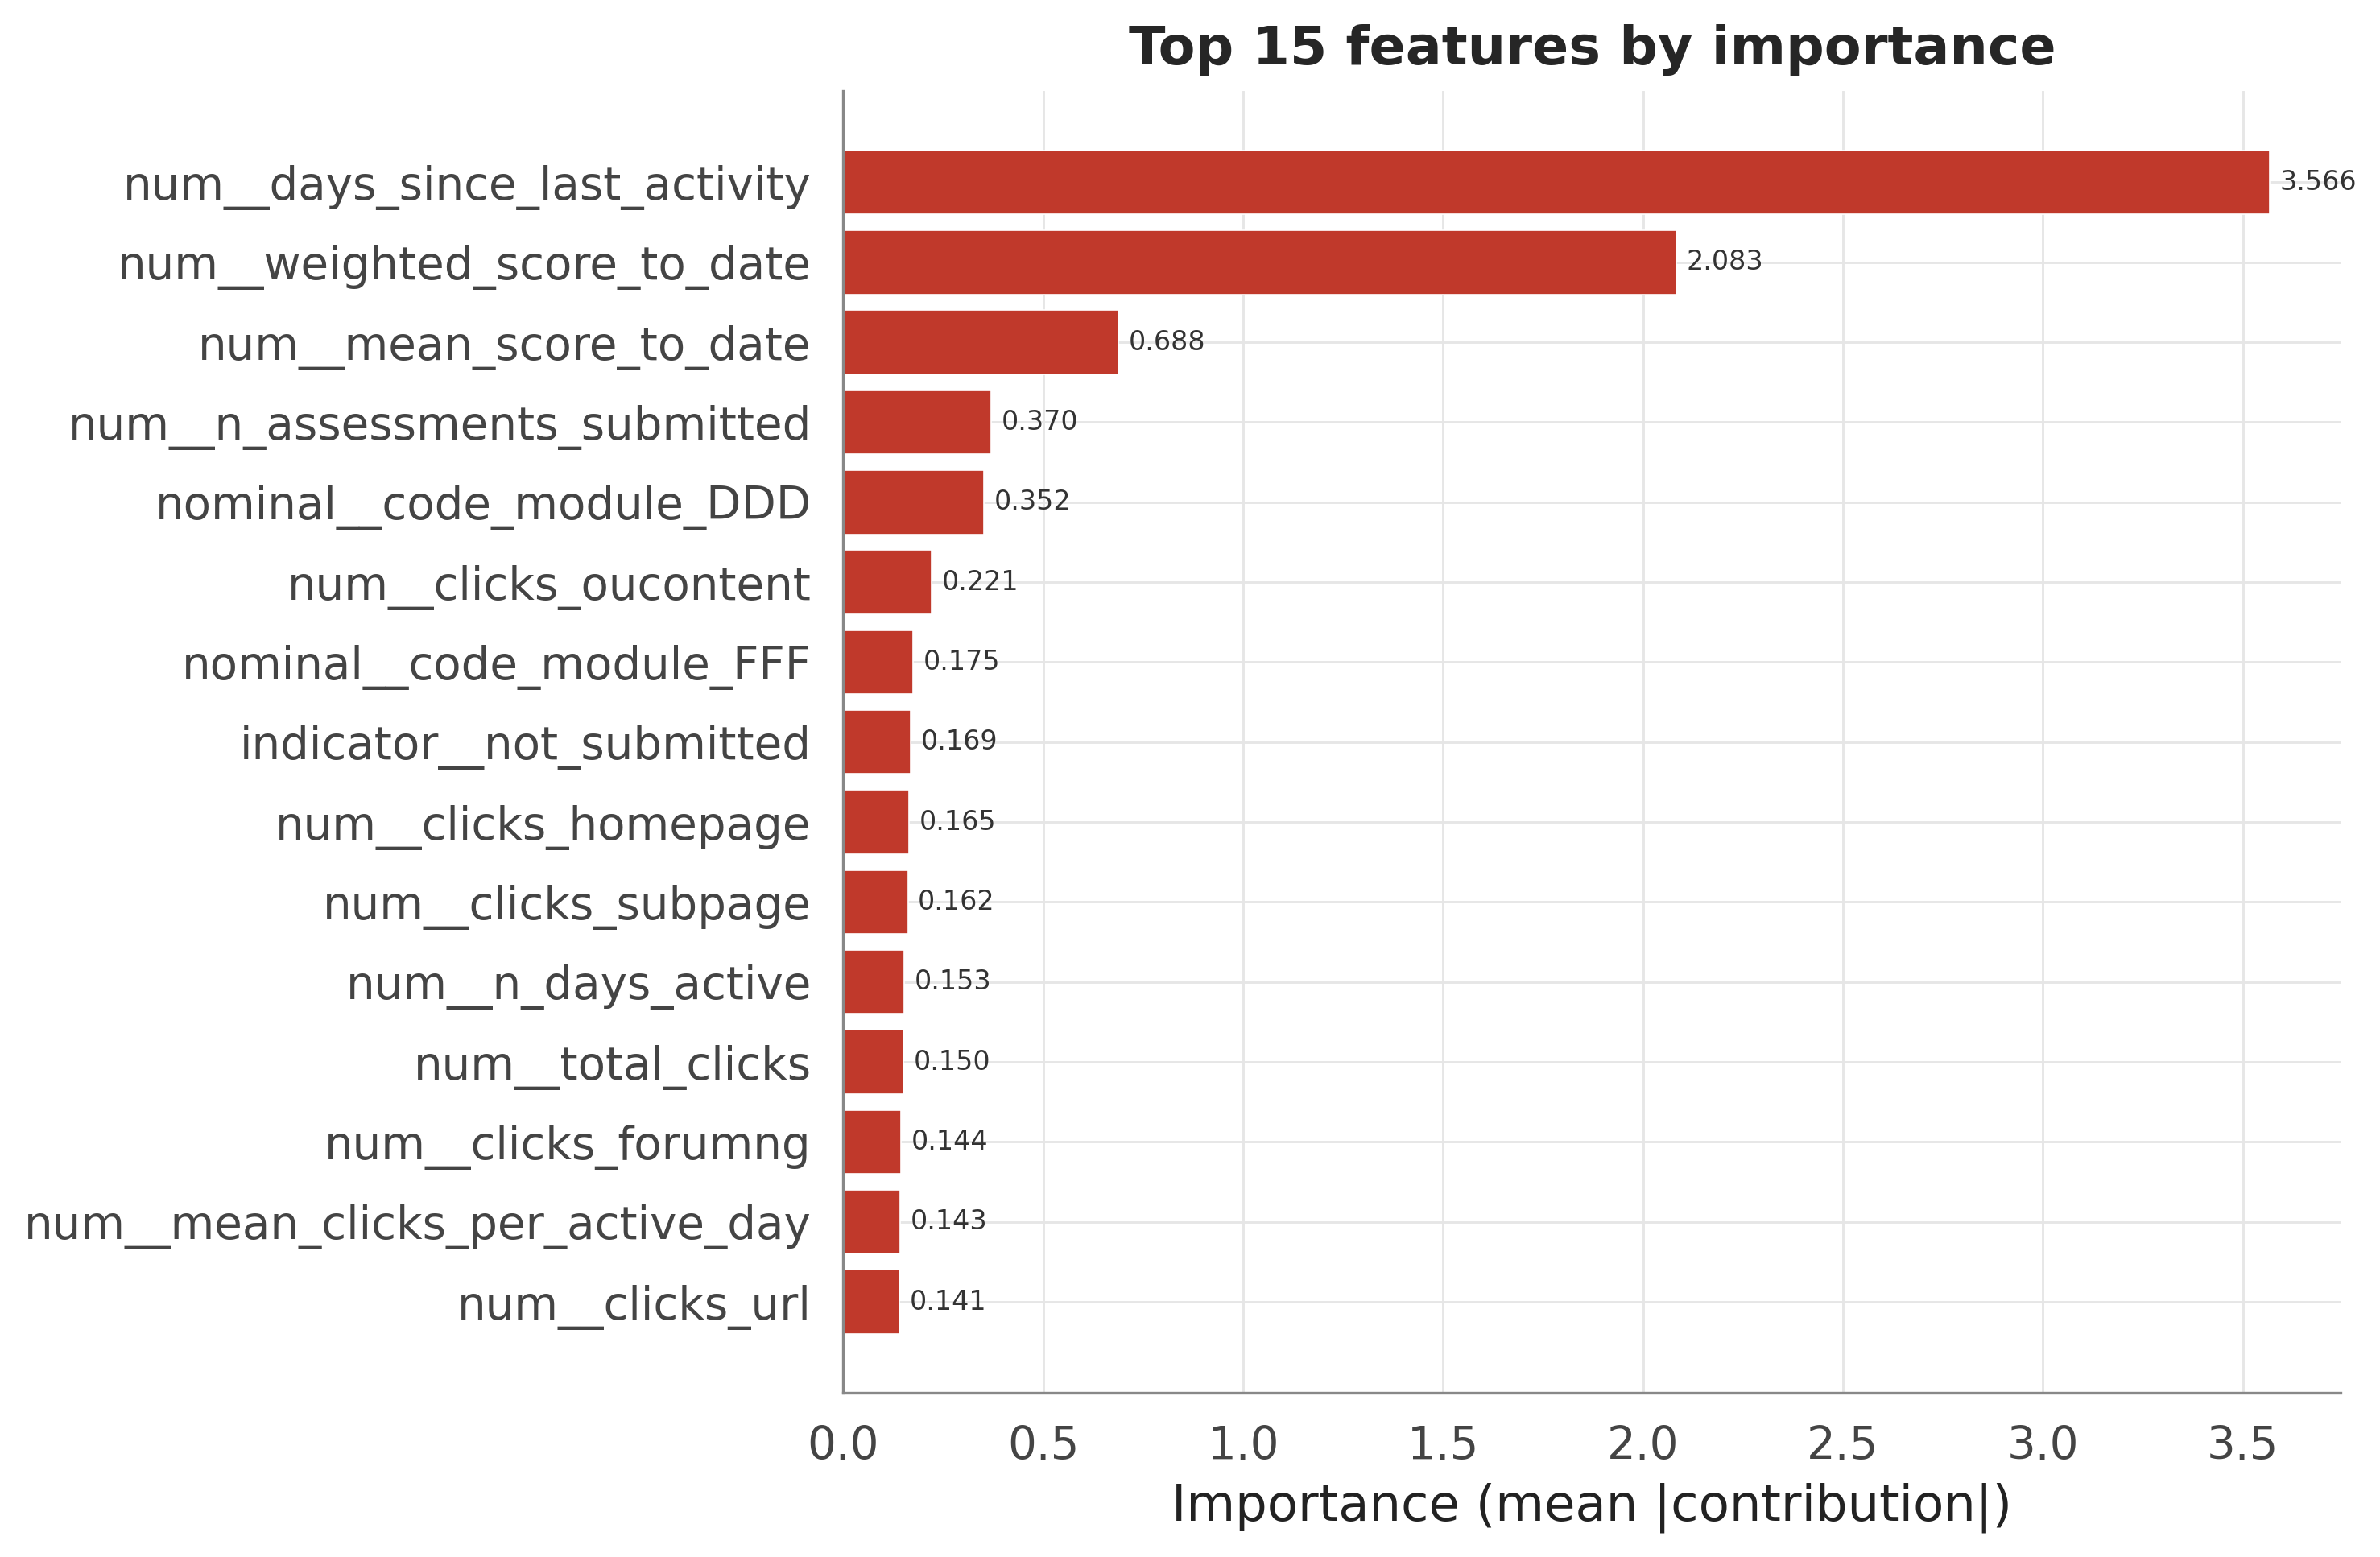
\includegraphics[height=0.76\textheight]{shap_importance_xgb_t100.png}\\
{\small Hai đặc trưng có đóng góp lớn nhất: \texttt{days\_since\_last\_activity} (3.57, số ngày kể từ lần hoạt động gần nhất) và \texttt{weighted\_score\_to\_date} (2.08, điểm đánh giá tích lũy có trọng số).}
\end{frame}

\begin{frame}{RQ2 · Độ ổn định của giải thích qua các mốc thời gian}
\centering
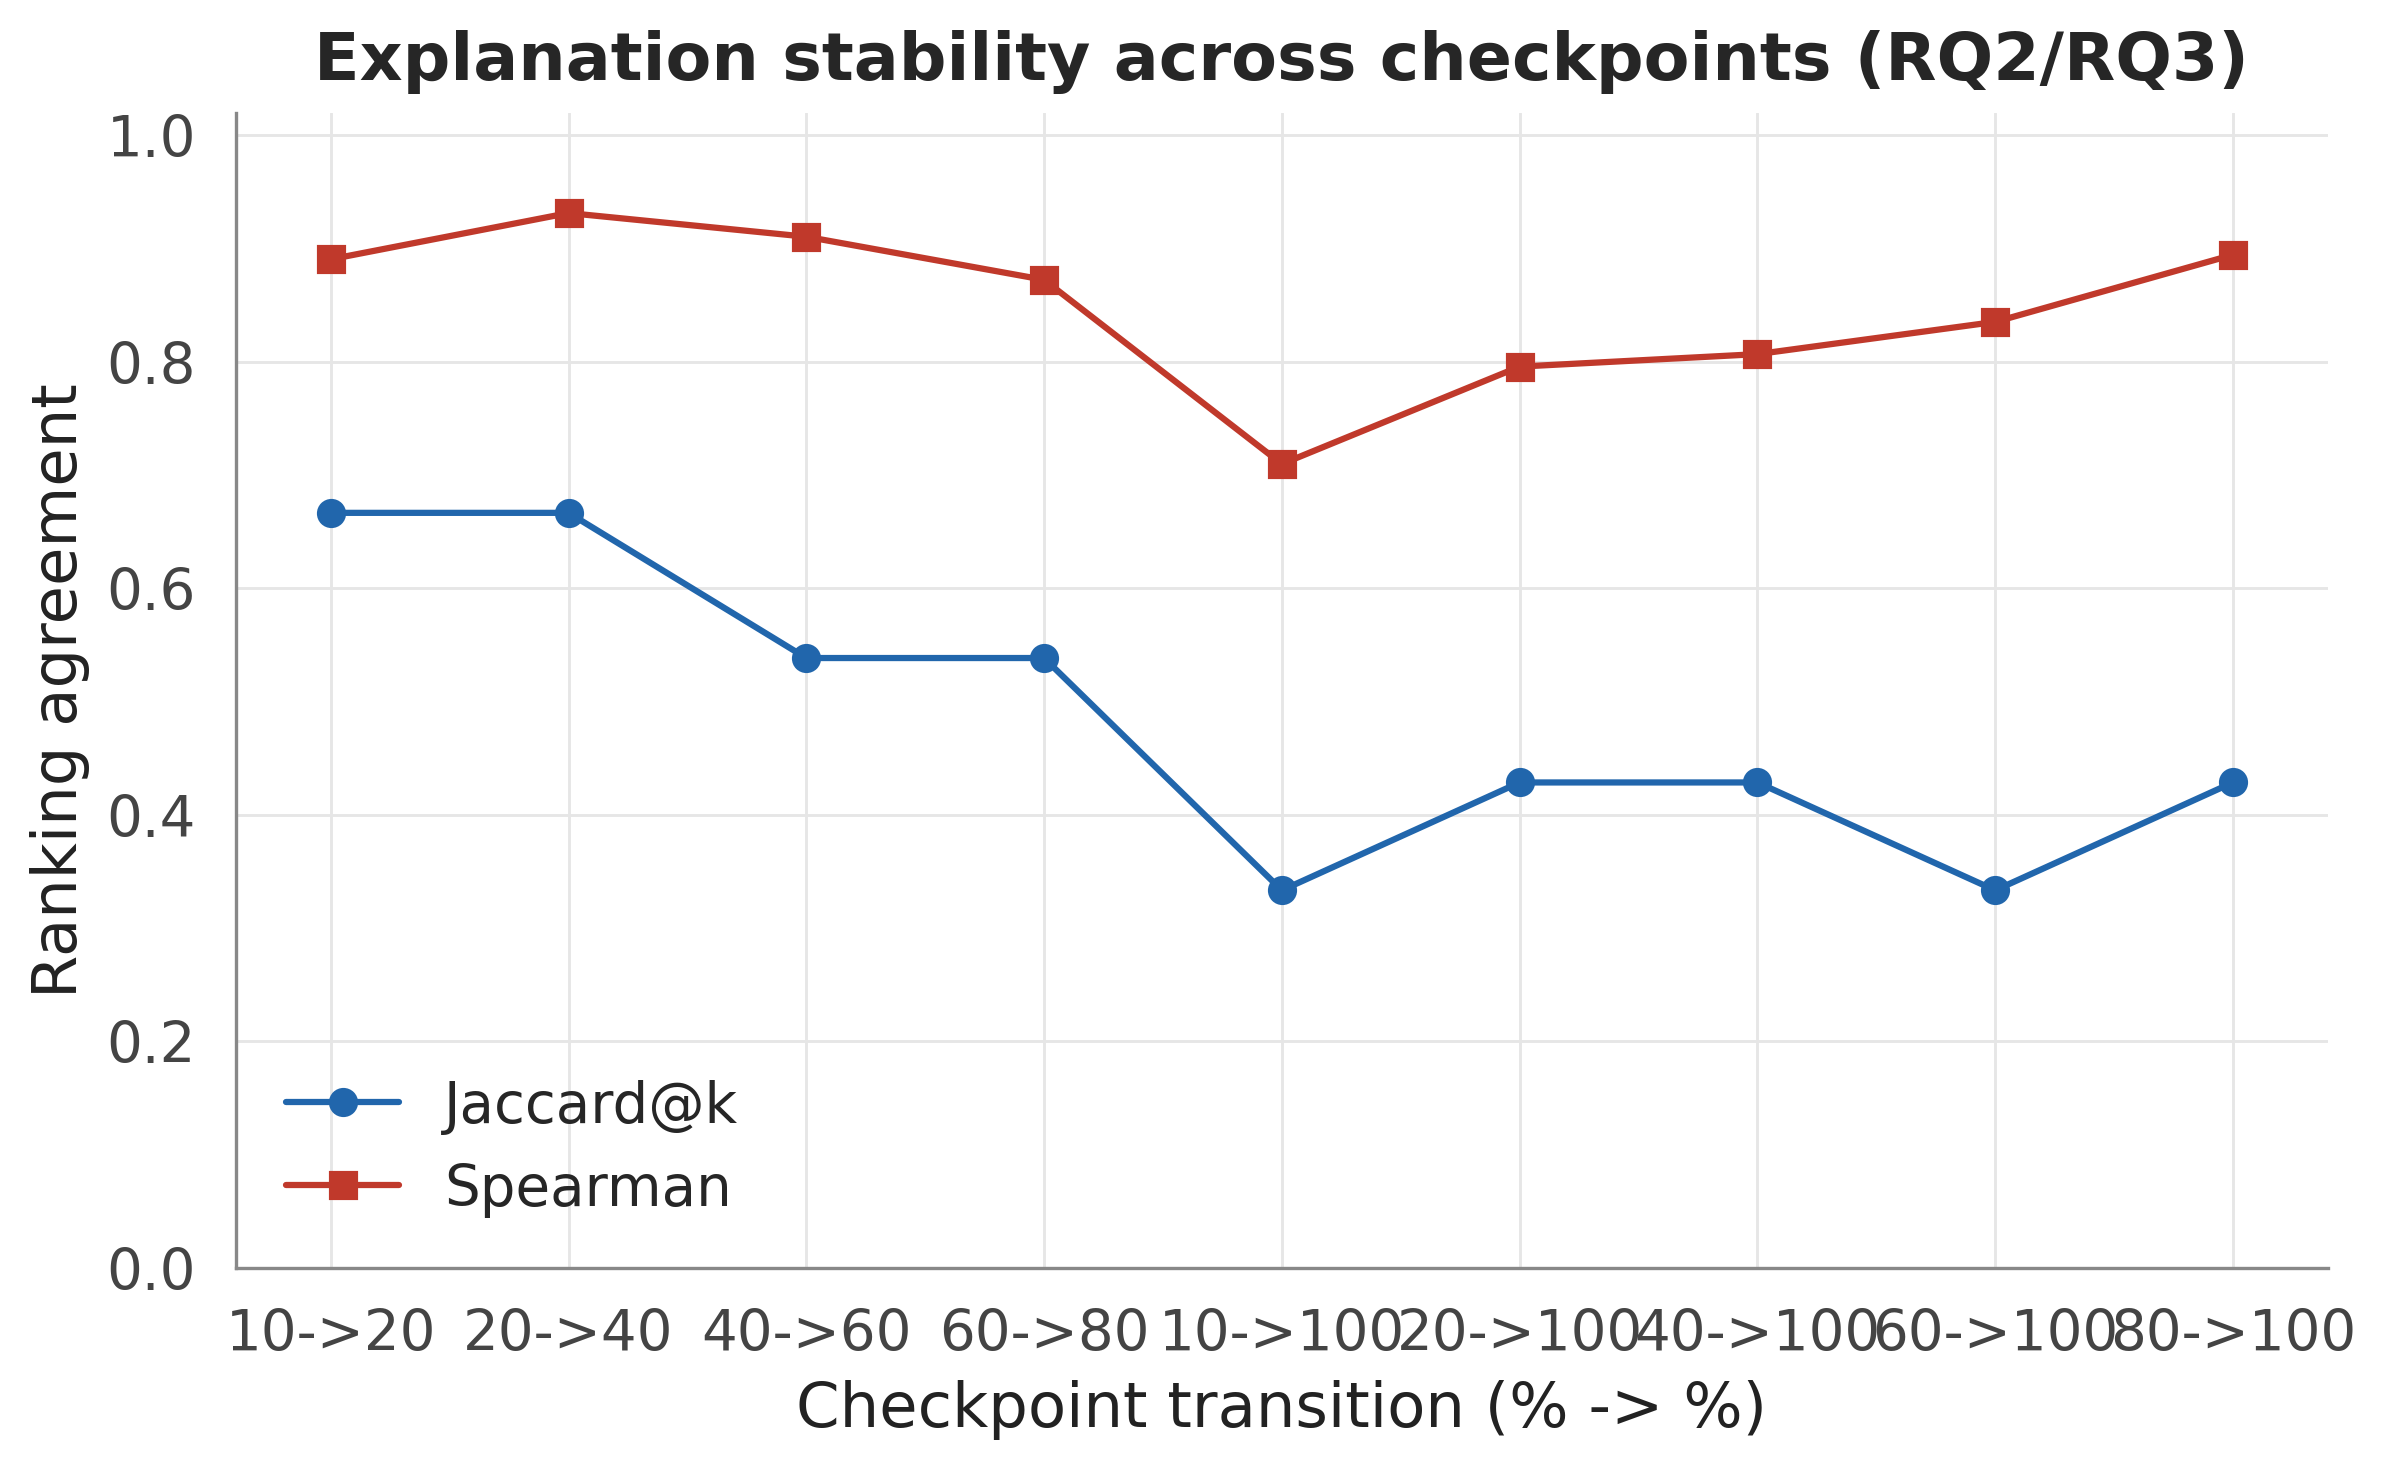
\includegraphics[height=0.76\textheight]{xai_stability_drift.png}\\
{\small Mức đồng thuận cao giữa các mốc liền kề và giảm dần khi khoảng cách thời gian giữa hai mốc tăng.}
\end{frame}

\begin{frame}{RQ2 · Định lượng độ ổn định, đối chiếu với mốc ngẫu nhiên}
\centering\small
\begin{tabular}{@{}lll@{}}
\toprule
\textbf{Phép đo} & \textbf{Kết quả} & \textbf{Đối chiếu mốc ngẫu nhiên} \\
\midrule
    Jaccard top 10 giữa 5 seed & \textbf{0.69} & cao hơn p99 (0.333) \\
    Spearman toàn thứ hạng giữa 5 seed & 0.97 & không áp dụng \\
    Jaccard top 10, SHAP so với LIME & 0.43 & cao hơn p99 (0.333) \\
    Spearman giữa các mốc liền kề & 0.87 đến 0.93 & không áp dụng \\
    Jaccard giữa t=10\% và t=100\% & 0.33 & xấp xỉ p99 (0.333) \\
    Jaccard giữa 4 chiến lược cân bằng & 0.54 đến 0.82 & Spearman $\geq$ 0.96 \\
\bottomrule
\end{tabular}
\vspace{3mm}
\begin{itemize}\small
  \item Mốc ngẫu nhiên: hai tập 10 đặc trưng chọn ngẫu nhiên từ 49 đặc trưng có Jaccard trung bình 0.119, phân vị 99 là 0.333. Mọi mức đồng thuận quan sát được đều vượt phân vị này, do đó độ ổn định không thể quy cho ngẫu nhiên.
  \item SHAP và LIME đồng thuận ở nhóm đặc trưng dẫn đầu (Jaccard top 10 bằng 0.43); tương quan toàn thứ hạng thấp hơn (Spearman 0.17) do phần cuối thứ hạng của LIME kém ổn định, vì vậy chỉ nhóm đặc trưng dẫn đầu được dùng để diễn giải.
  \item Thành phần top 10 thay đổi dần theo thời gian (Jaccard giữa t=10\% và t=100\% bằng 0.33), phù hợp với kỳ vọng: tín hiệu giai đoạn sớm thiên về hành vi, giai đoạn cuối thiên về kết quả đánh giá.
\end{itemize}
\end{frame}

\begin{frame}{Kết luận Task 4: ba câu trả lời}
\begin{itemize}
  \item Năm thuật toán thuộc ba họ được so tuyển trong cùng điều kiện; \textbf{XGBoost} được chọn (recall baseline 0.931) với hai lớp kiểm chứng: kiểm định chéo 5 fold $\times$ 5 seed và kiểm định Friedman, Wilcoxon. Tinh chỉnh siêu tham số không mang lại cải thiện tương xứng, nên cấu hình gần mặc định được giữ nguyên.
  \item \textbf{RQ1, kết luận kép:} quần thể đầy đủ đạt chuẩn từ t=40\% ở mức ranh giới (khoảng tin cậy chứa 0,80); quần thể còn theo học chỉ đạt chuẩn tại t=100\%; chênh lệch giữa hai quần thể có ý nghĩa thống kê tại cả sáu mốc.
  \item \textbf{RQ3:} bốn chiến lược cân bằng lớp chênh nhau tối đa 0.0069 recall; kết quả bền vững, không phụ thuộc cách xử lý mất cân bằng.
  \item \textbf{RQ2:} độ ổn định của giải thích vượt phân vị 99 của mốc ngẫu nhiên (Jaccard giữa các seed 0.69 so với 0.333); SHAP và LIME đồng thuận ở nhóm đặc trưng dẫn đầu.
  \item Toàn bộ slide và kịch bản sinh lại từ CSV bằng lệnh \texttt{python -m tools.build\_task4\_slides}.
\end{itemize}
\vspace{2mm}
\centering\color{themecol}\textbf{Nhóm 5 xin cảm ơn thầy cô và các bạn!}
\end{frame}

\end{document}
